\documentclass[logo,magister]{tesis-postgrado}

% % Declaración para colocar código Java
%\usepackage{listings}
%\usepackage{color}
%
%\definecolor{dkgreen}{rgb}{0,0.6,0}
%\definecolor{gray}{rgb}{0.5,0.5,0.5}
%\definecolor{mauve}{rgb}{0.58,0,0.82}
%
%\lstset{frame=tb,
%  captionpos=b, 
%  language=Java,
%  numbers=left,
%  aboveskip=3mm,
%  belowskip=3mm,
%  showstringspaces=false,
%  columns=flexible,
%  basicstyle={\small\ttfamily},
%  %numbers=none,
%  numberstyle=\tiny\color{gray},
%  keywordstyle=\color{blue},
%  commentstyle=\color{dkgreen},
%  stringstyle=\color{mauve},
%  breaklines=true,
%  breakatwhitespace=true,
%  tabsize=3
%}

\renewcommand{\lstlistingname}{C\'ODIGO}

% % Pa usar quotes
\usepackage{csquotes}

\keywords{XML; Key Implication}

\begin{document}
\baselineskip 23pt
% ----------------------------------------------------------
\thispagestyle{empty}
\titulo{Estrategias de planificación para motores de búsqueda verticales}

\autor{Danilo Fernando Bustos Pérez}

\fecha{Lunes}{15}{Enero}{2014} %Del Examen de Grado

\profesorguia{Dra.\ Carolina Bonacic Castro}

\profesorcoguia{Dr.\ Mauricio Marín Caihuán}

\ciudad{Santiago}
\pais{Chile}
\makecubierta
\makecopyright
% ----------------------------------------------------------
\frontmatter

\begin{gracias}

Agradecimientos...


\end{gracias}
% % AGREGADO PARA IMPRIMIR EN DOBLE CARA
\newpage\null\thispagestyle{empty}\newpage
\dedicatoria{
	Para Rubén, Flor, familia y amigos
}
% % AGREGADO PARA IMPRIMIR EN DOBLE CARA
\newpage\null\thispagestyle{empty}\newpage

\resumenCastellano{
La flexibilidad sintáctica, y el complejo anidamiento de los datos en una estructura tipo árbol 
dificulta expresar propiedades deseables de los datos XML, ofreciendo una capacidad limitada para 
expresar semántica. En esta tesis se presenta un estudio de las claves como restricciones de 
integridad sobre documentos XML, implementando algoritmos para los problemas de implicación y 
validación, con el fin de mostrar la factibilidad de usar las capacidades semánticas que éstas 
entregan, y que XML como modelo requiere.
\vspace*{0.5cm}
\KeywordsES{XML; Claves XML; Implicación de claves; Validación de documentos XML; Cover no redundante}
}

\newpage

\resumenIngles{
The syntactic flexibility and complex tree-like nested data make it challenging to express desirable 
properties of XML data, offering a limited capability to express semantic. In this thesis, we present 
a study of keys as integrity constraints on XML documents, implementing algorithms for implication 
and validation problems, with the aim of showing the factibility of using the semantic capabilities 
that keys gives and XML as a model requires.
\vspace*{0.5cm}
\KeywordsEN{XML; XML keys; Key implication; XML document validation; Non-redundant cover}
}

\pagestyle{fancy}
\fancyhead[L]{\slshape \leftmark}
\fancyhead[C]{}
\fancyhead[R]{\thepage}
\pagenumbering{roman}
\tableofcontents
\listoffigures
\listoftables
% % AGREGADO PARA IMPRIMIR EN DOBLE CARA
\newpage\null\thispagestyle{empty}\newpage
%\listofalgorithms
% ----------------------------------------------------------
\mainmatter
\fancyhead[L]{\slshape \leftmark}
\fancyhead[C]{}
\pagenumbering{arabic}
\hyphenation{de-di-ca-da a-no-ta-cio-nes re-sul-ta-dos fun-cio-na-les se-man-ti-ca}
\chapter{Introducci\'on}
\label{cap:intro}


% ***************************************************************************************************** MOTIVACIÓN

\section{Antecedentes y motivaci\'on}
\label{intro:motivacion}



\section{Descripci\'on del problema}
\label{intro:problema}




\section{Objetivos y solución propuesta}


\subsection{Objetivo General}


\subsection{Objetivos Espec\'ificos}


\subsection{Alcances}



\subsection{Soluci\'on propuesta}
\label{intro:solucionpropuesta}



\subsection{Caracter\'isticas de la solución}
\label{intro:caracteristicassolucion}


\subsection{Prop\'osito de la solución}
\label{intro:propositosolucion}



\section{Metodolog\'ia y herramientas de desarrollo}
\subsection{Metodolog\'ia}



\subsection{Herramientas de desarrollo}


\section{Resultados obtenidos}


\section{Organizaci\'on del documento}


\chapter{Marco te\'orico}
\label{cap:marco}
En este capítulo se exponen los conceptos teóricos del presente trabajo de tesis. Primero se explica qué es un motor de búsqueda vertical. Luego se definen las estrategias de evaluación de transacciones de lectura, también conocidas como consultas o \textit{queries}. Posteriormente se describen las diferentes operaciones sobre listas invertidas. Finalmente se explica el concepto de \textit{ranking}. 

\section{Motores de búsqueda verticales}
\label{marco:mbv}
Un motor de búsqueda está construído por diversos componentes, su arquitectura típica se puede ver en la Figura \ref{fig:searchenginearchitecture}. Existe un proceso denominado \textit{crawling}, éste posee una tabla con los documentos iniciales en los que se extrae el contenido de cada uno de ellos. A medida que el \textit{crawler} comienza a encontrar enlaces a otros documentos, la tabla de documentos a visitar crece. El contenido que se extrae en el procedimiento de \textit{crawling} es enviado al proceso de indexamiento, este se encarga de crear un índice de los documentos ya visitados por el \textit{crawler} \citep{Croft:2009}.

\begin{figure}[!th]
\centering
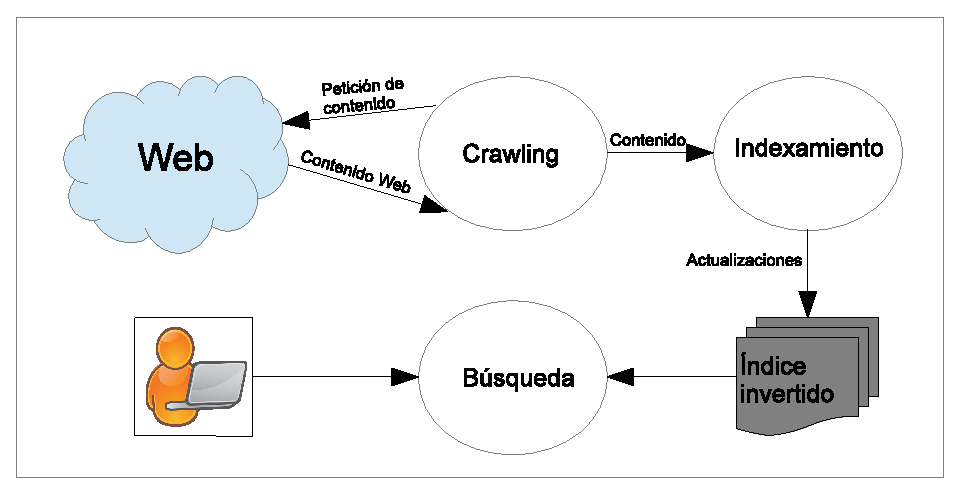
\includegraphics[scale=.75]{images/searchenginearchitecture.eps}
\caption{Arquitectura típica de un motor de búsqueda}
\label{fig:searchenginearchitecture}
\end{figure}

Dado el volúmen de datos involucrado en el procesamiento, se debe tener una estructura de datos que permita encontrar cuáles documentos contienen las palabras presentes en la búsqueda que llega al sistema. Todo esto dentro de un período de tiempo aceptable. El índice invertido \citep{Zobel:2006} es una estructura de datos que contiene un diccionario con todas las palabras que el proceso de \textit{crawling} ha encontrado, asociado a cada palabra se tiene una lista de todos los documentos en donde esta palabra aparece mencionada (conocida como lista invertida de un término). El motor de búsqueda construye esta estructura con el objetivo de acelerar el proceso de las búsquedas que llegan al sistema. El proceso de búsqueda es el encargado de recibir las transacciones de lectura, generar un \textit{ranking} de los documentos que contienen las palabras de la consulta y finalmente generar una respuesta. Las diversas formas de calcular la relevancia de un documento será explicado en secciones posteriores.

En un motor de búsqueda se pueden encontrar diversos servicios tales como (a) cálculo de los mejores documentos para una cierta consulta; (b) construcción de la página Web en la que se mostrará al usuario los resultados; (c) publicidad relacionada con las transacciones de lectura; (d) sugerencias en el momento que el usuario está escribiendo la consulta en el sistema; entre muchos otros servicios.

En los sistemas de recuperación de información como los motores de búsqueda, lo que se hace hoy en día es agrupar computadores para procesar una transacción y obtener la respuesta para ésta. Este conjunto de computadores recibe el nombre de \textit{cluster} \citep{Dean:2009}.

La diferencia entre un motor de búsqueda vertical y uno general, es que el primero se centra solo en un contenido específico de la Web \citep{Gil-Costa:2013}. El \textit{crawler} debe extraer contenido solo de aquellas páginas Web que están dentro del dominio permitido. Al ser un dominio acotado, los documentos a procesar serán menos y por lo tanto, la lista de los términos del índice invertido serán eventualmente de menor tamaño. Sin embargo, en un motor de búsqueda vertical las actualizaciones al índice invertido ocurren con mayor frecuencia.

\section{\'Indice invertido}
\label{marco:ii}
Es una estructura de datos que contiene todos los términos (palabras) encontrados por el \textit{crawler}. A cada uno de los términos está asociado una lista invertida de documentos (páginas Web) que contienen dicho término. Adicionalmente, se almacena información que permita realizar el \textit{ranking} de documentos para generar la respuesta a las consultas que llegan al sistema, por ejemplo, el número de veces que aparece el término en el documento.

Para construir un índice invertido \citep{Baeza-Yates:2011, Salton:2003} se debe procesar cada palabra que existe en un documento, registrando su posición y la cantidad de veces que éste se repite. Cuando se procesa el término con la información asociada correspondiente, se almacena en el índice invertido (ver Figura \ref{fig:invertedindex}).

\begin{figure}[!th]
\centering
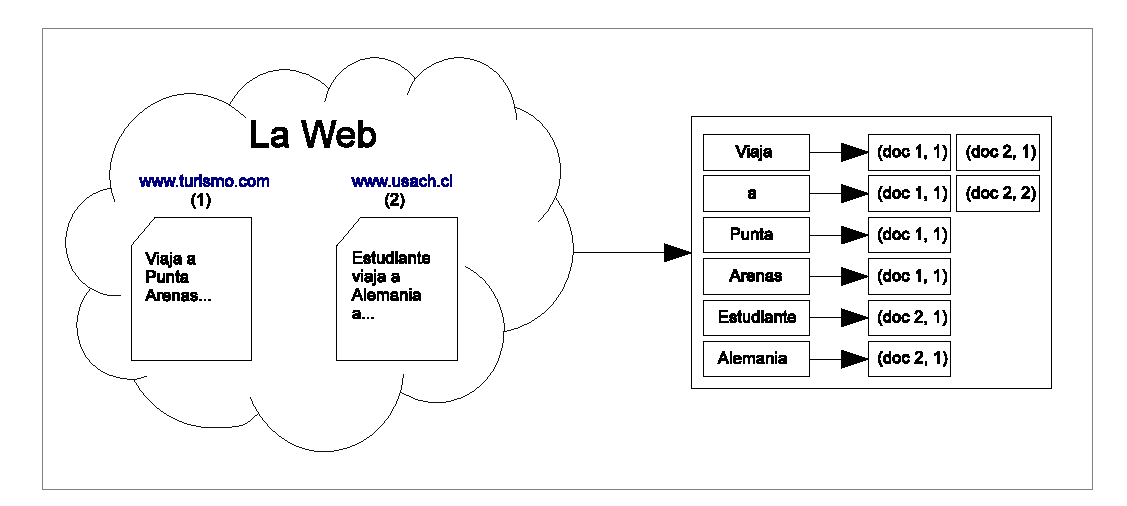
\includegraphics[scale=.75]{images/invertedindex.eps}
\caption{\'Indice invertido}
\label{fig:invertedindex}
\end{figure}

El tamaño del índice invertido crece rápido y eventualmente la memoria RAM se agota antes de procesar toda la colección de documentos. Cuando la memoria RAM se agota, se almacena en disco el índice parcial, se libera la memoria y se continúa con el proceso. Además, se debe hacer un \textit{merge} de los índices parciales uniéndo las listas invertidas de cada uno de los términos involucrados. Es por esto que se han desarrollado algunas técnicas de compresión con el objetivo de guardar de una manera más eficiente el índice invertido \citep{Arroyuelo:2013, Baeza-Yates:2011, Yan:2009}.

\section{Estrategias de evaluaci\'on de transacciones de lectura}
\label{marco:eeq}
Una de las tareas que un motor de búsqueda debe hacer para resolver una consulta es calcular el puntaje o \textit{score} para aquellos documentos relevantes en la consulta y así poder extraer los mejores $K$ documentos. Existen dos principales estrategias para recorrer las listas invertidas y calcular el puntaje de los documentos para una determinada consulta. Estas son (a) \textit{term-at-a-time} \citep{Buckley:1985, Turtle:1995} y (b) \textit{document-at-a-time} \citep{Broder:2003, Turtle:1995}.

\subsection{\textit{Term at a time}}
\label{marco:TAAT}
Abreviada TAAT, este tipo de estrategia procesa los términos de las consultas una a una y acumula el puntaje parcial de los documentos. Las listas invertidas asociadas a un término son procesadas secuencialmente, esto significa que todos los documentos presentes en la lista invertida del término $t_{i}$ obtienen un puntaje parcial antes de comenzar el procesamiento del término $t_{i+1}$. La secuencialidad en este caso es con respecto a los términos contenidos en la transacción de lectura.

\subsection{\textit{Document at a time}}
\label{marco:DAAT}
Abreviada DAAT, en este tipo de estrategias se evalúa la contribución de todos los términos de la transacción de lectura con respecto a un documento antes de evaluar el siguiente documento. Las listas invertidas de cada término de la consulta son procesadas en paralelo, de modo que el puntaje del documento $d_{j}$ se calcula considerando todos los términos de la transacción de lectura al mismo tiempo. Una vez que se obtiene el puntaje del documento $d_{j}$ para la consulta completa, se procede al procesamiento del documento $d_{j+1}$. Este tipo de estrategia posee dos grandes ventajas: (a) Requieren menor cantidad de memoria para su ejecución, ya que el puntaje parcial por documento no necesita ser guardado y (b) Explotan el paralismo de entrada y salida (I/O) más eficientemente procesando las listas invertidas en diferentes discos simultáneamente.

\section{Funciones de \textit{Ranking}}
\label{marco:ranking}
Los sistemas de recuperación de información como los motores de búsqueda deben ejecutar un proceso el cual asigna puntaje a documentos con respecto a una determinada transacción de lectura, este proceso se denomina \textit{ranking} \citep{Baeza-Yates:2011}. Como se puede ver en la Figura \ref{fig:ranking_process}, este proceso toma como entrada la representación de las consultas y documentos, y asigna un \textit{score} a un documento $d_{j}$ dada una consulta $q_{i}$.

Un motor de búsqueda guarda billones de documentos que están formados por términos o palabras, estos términos no todos poseen la misma utilidad para describir el contenido del documento. Determinar la importancia de una palabra en un documento no es tarea sencilla, para ello se asocia un peso positivo $w_{i,j}$ a cada término $t_{i}$ del documento $d_{j}$. De esta forma, para un término $t_{i}$ que no aparezca en el documento $d_{j}$ se tendrá $w_{i,j} = 0$. La asignación de pesos a los términos permite generar un \textit{ranking} numérico para cada documento en la colección.

\begin{figure}[!th]
\centering
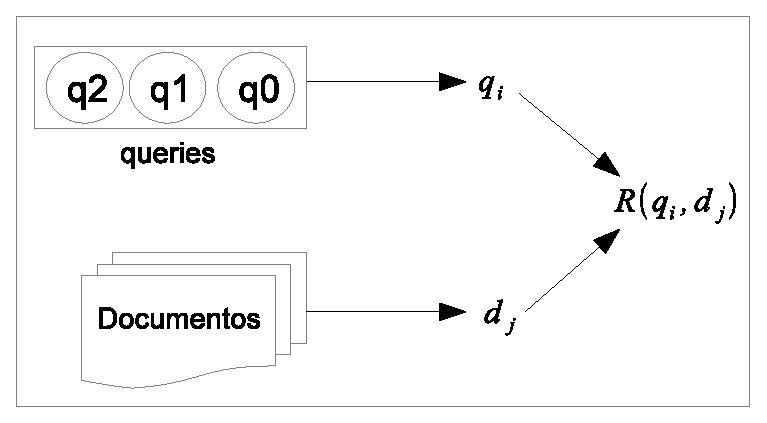
\includegraphics[scale=.75]{images/ranking_process.eps}
\caption{Proceso de \textit{scoring} de documento}
\label{fig:ranking_process}
\end{figure}

\subsection{TF-IDF}
\label{marco:tfi-df}
$Tf-idf$ (\textit{term frequency - inverse document frequency}) es un estadístico que tiene por objetivo reflejar cuán importante es una palabra para un documento en una colección o corpus %. Este estadístico se divide en dos partes, el primero corresponde a la frecuencia del término en un documento ($tf$) y que en su versión más sencilla se utiliza la frecuencia bruta del término $t$ en el documento $d$ ($f(t,d)$) dividido por la frecuencia de la palabra que más se repite en el documento $d$.  

\begin{equation}
\label{formula:tf}
tf(t,d) = \dfrac{f(t,d) }{ \max{f(w,d) : w \in d}}
\end{equation}

El segundo término corresponde a la frecuencia inversa de documento ($idf$) y se utiliza para observar si es que el término es común en el corpus. El $idf$ se obtiene calculando el logaritmo de la división entre el número total de documentos del corpus y el número de documentos que contienen el término.

\begin{equation}
\label{formula:idf}
idf(t,D) = log \frac{ |D| }{1 + |{d \in D : t \in d}|}
\end{equation}

De esta forma a partir de \eqref{formula:tf} y \eqref{formula:idf} se obtiene finalmente el $tf-idf$: 

\begin{equation}
\label{formula:tfi-df}
tf-idf(t,d,D) = tf(t,d) * idf(t,D)
\end{equation}

Notar en \eqref{formula:tfi-df} que el estadístico incrementa proporcionalmente al número de veces que la palabra aparece en el documento, sin embargo, es compensado por la frecuencia de la palabra en la colección completa de documentos o corpus. Esta compensación ayuda a controlar el hecho de que algunas palabras son generalmente más comunes que otras.


\subsection{BM25}
\label{marco:bm25}
Es una función de \textit{ranking} de documentos basada en los términos que aparecen en la consulta que llega al motor de búsqueda. \textit{BM25} pertenece a una amplia gama de funciones de puntuación y está basada en los modelos probabilísticos de recuperación de la información \citep{Baeza-Yates:2011}.

Dada una consulta $Q$ que contiene los términos $q_{1},...,q_{n}$, el \textit{ranking BM25} del documento D se calcula como: 

\begin{equation}
\label{formula:bm25}
score(D,Q) =  \displaystyle\sum_{i=1}^n IDF(q_{i}) * \frac{f(q_{i},D)*(k+1)}{f(q_{i},D)+k * (1 - b + b * \frac{|D|}{prom(docs)})}
\end{equation}

En donde: $f(q_{i}, D)$ es la frecuencia en que aparece el término $q_{i}$ en el documento D; $|D|$ es el número de palabras o términos en el documento D; $prom(docs)$ es la media de número de palabras de los documentos en el corpus; k y b son constantes que depende de las características del corpus en el que se está haciendo la búsqueda, por lo general se asignan los valores de $k = 2$ o $k = 1.2$ y $b = 0.75$; finalmente, $IDF(q_{i})$ es la frecuencia inversa de documento para el término $q_{i}$.


\section{Operaciones sobre listas invertidas}
\label{marco:osli}
Cuando una consulta llega al motor de búsqueda, cada término tiene asociado una lista con todos los documentos en los cuales aparece. El sistema debe decidir qué documentos se analizarán para obtener la respuesta y entregar al usuario una respuesta. A continuación se presenta los modos de operar las listas invertidas para una cierta transacción de lectura.

\subsection{\textit{OR}}
\label{marco:or}
Este operador toma las listas invertidas de cada uno de los términos de la transacción de lectura y ejecuta la disyunción entre ellas. El resultado de este operador es una lista invertida con todos los documentos que contengan al menos un término de la consulta. Finalmente, esta lista invertida se ocupará para obtener los mejores K documentos. Un simple ejemplo se muestra en la Figura \ref{fig:ORoperation}.

\begin{figure}[!th]
\centering
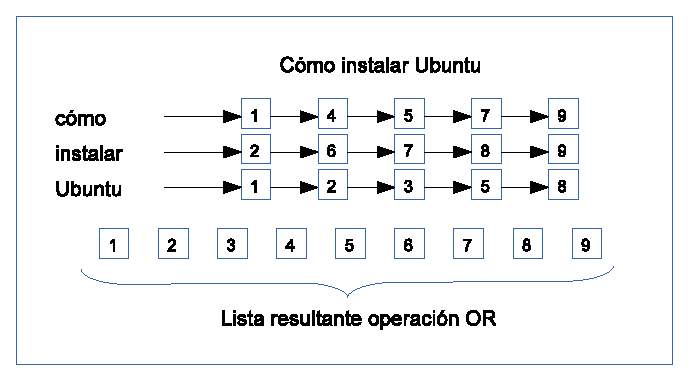
\includegraphics[scale=.75]{images/ORoperation.eps}
\caption{Operaci\'on OR}
\label{fig:ORoperation}
\end{figure}

\subsection{AND}
\label{marco:and}
Este operador ejecuta la conjunción entre las listas invertidas de los términos de una transacción de lectura. Se obtiene una lista invertida con los documentos que contengan todos los términos de la consulta. Se debe notar que aquí se obtiene una lista resultante de menor tamaño que la obtenida en el operador OR (Ver Figura \ref{fig:ANDoperation}).

\begin{figure}[!th]
\centering
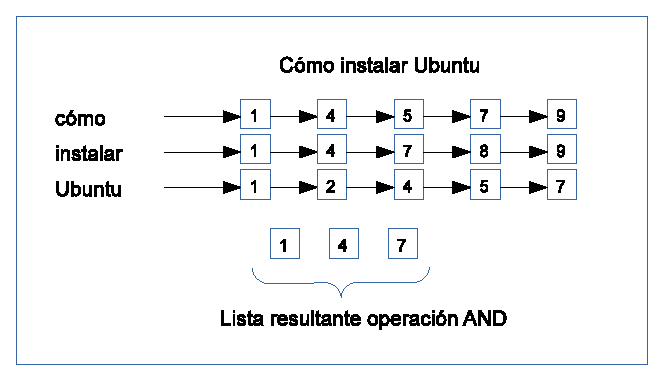
\includegraphics[scale=.75]{images/ANDoperation.eps}
\caption{Operaci\'on AND}
\label{fig:ANDoperation}
\end{figure}

\subsection{Wand}
\label{marco:wand}
Algoritmo de evaluación de transacciones de lectura para obtener eficientemente el conjunto de $K$ documentos que mejor satisfacen una consulta dada. WAND \citep{Broder:2003} es un proceso menos estricto que el método \textit{AND} y está basado en dos niveles. Dentro del proceso de evaluación de una transacción de lectura, uno de los procesos más costoso en términos de tiempo es el de \textit{scoring}, que consiste en entregarle a cada uno de los documentos analizados un puntaje que representa la relevancia del documento para una transacción de lectura dada, esto se denomina evaluación completa o cálculo del puntaje exacto del documento. El objetivo de WAND es minimizar la cantidad de evaluaciones completas de los documentos ejecutando un proceso de dos niveles. En el primer nivel se intenta omitir rápidamente grandes porciones de las listas invertida, lo que se traduce en ignorar el cálculo del puntaje exacto de grandes cantidades de documentos, esto porque en motores de búsqueda a gran escala, este un proceso que requiere de mucho tiempo para llevarse a cabo y depende de factores como la cantidad de ocurrencia del término dentro del documento, el tamaño del documento, entre otros. A este tipo de técnicas que intenta omitir partes de lista invertida se les conoce como técnica de poda dinámica \citep{Broder:2003, Persin:1994, Turtle:1995}. 

Para llevar a cabo el algoritmo WAND y así reducir el número de documentos completamente evaluados durante el proceso de \textit{ranking} de documentos, se necesita calcular los valores estáticos de límite superior (\textit{upper-bounds}), en donde para cada uno de los términos del índice invertido, se toma la lista invertida correspondiente y se extrae el puntaje máximo de contribución de algún documento con respecto al término. El cálculo de los \textit{upper bounds} se lleva a cabo cuando se construye el índice invertido y en donde a cada término del índice se asocia el puntaje máximo que existe en la lista invertida. 

WAND usa un índice invertido ordenado por los identificadores de documentos. En el primer nivel se itera sobre los documentos del índice invertido de cada término y se identifican los potenciales candidatos usando una evaluación aproximada. En el segundo nivel, aquellos documentos candidatos son completamente evaluados y su puntaje exacto es calculado. De esta forma se obtiene el conjunto final de documentos. Se utiliza un heap como estructura de datos para almacenar el conjunto de los mejores $K$ documentos, en donde el elemento superior corresponde al documento con menor puntaje y es el que se utilizará como umbral (\textit{threshold}) para decidir si los siguientes documentos deben ser completamente evaluados o no.

En la Figura \ref{fig:proceso_wand} se puede ver un ejemplo sencillo de cómo el algoritmo Wand trabaja en la resolución de una transacción de lectura de tres términos: 'casa', 'perro' y 'gato'. Como la consulta está compuesta por tres términos, existen tres punteros que recorren cada una de las listas invertidas (notar que cada puntero recorre una lista invertida diferente). Lo primero que se hace es ordenar las listas invertidas de acuerdo a los identificadores de documentos que se están apuntando, razón por la cual en la Figura \ref{fig:proceso_wand} la lista invertida de 'casa' (puntero referenciando al documento con identificador 125), aparece primero que la lista invertida de 'perro' (puntero haciendo referencia al documento con identificador 503). Luego se suma los \textit{uppers bounds} de los términos en orden hasta que se obtiene un valor mayor o igual al \textit{threshold}. De esta manera el término 'perro' es escogido como término pivote ($2.0 + 4.4 \geq 5.7$) y el actual documento al cual se está apuntando es escogido como documento pivote (documento con identificador 503). Si las dos primeras listas invertidas no contienen el documento 503 entonces se procede a seleccionar el siguiente pivote, en otro caso se calcula el puntaje completo del documento. Finalmente, si el puntaje es mayor o igual al \textit{threshold}, se actualiza el \textit{heap} eliminando el elemento superior y se añade el nuevo documento. 
Este algoritmo es repetido hasta que no hayan más documentos a procesar o hasta que no exista un documento que supere el actual \textit{threshold}. De esta manera se evita procesar las listas completas \citep{Blanco:2010}.

\begin{figure}[!th]
\centering
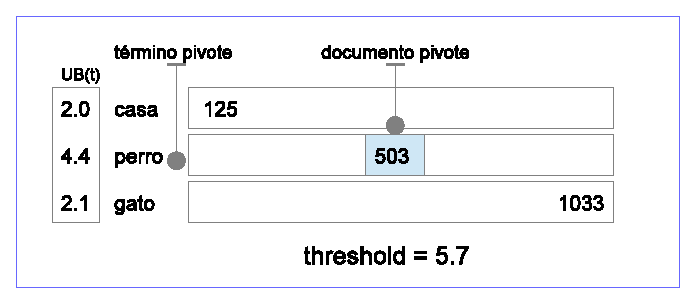
\includegraphics[scale=.75]{images/proceso_wand.eps}
\caption{Ejemplo de ejecución de algoritmo Wand}
\label{fig:proceso_wand}
\end{figure}

\subsection{Block Max Wand}
\label{marco:bmw}
Como se explicó en la sección anterior, la diferencia entre un método exhaustivo de evaluación de documentos y el método Wand, es que este último es una técnica DAAT de poda dinámica \citep{Moffat:1996} en la que se intenta omitir la mayor cantidad de evaluaciones de documentos haciendo uso de una estrategia de movimientos de punteros pivotes.
Bajo la premisa que Wand tradicional es limitado por el hecho que usa los máximos puntajes de las listas invertidas (\textit{Upper bounds}) para podar, puesto que estos pueden ser mucho más grandes que el promedio de puntaje en ellas, se propone un método llamado \textit{Block-Max-Wand} (BMW) \citep{Ding:2011}. Este método utiliza una estructura de datos llamada índice \textit{Block-Max}, en donde el índice invertido estará particionado en bloques y para cada bloque se almacena la máxima contribución de algún documento dentro del bloque. En otras palabras, se tendrán tantos \textit{upper bounds} locales como bloques existan en la lista invertida.

Este método utiliza una variación del algoritmo Wand tradicional para que trabaje correctamente con la nueva estructura \textit{Block-Max-Wand}. Remplazar el uso de los \textit{upper bounds} de cada bloque por el \textit{upper bound} global no garantiza la correctitud del algoritmo. En la Figura \ref{fig:bmw} se muestra un ejemplo de por qué mirar solo los \textit{upper bounds} locales no garantiza obtener los resultados correctos, aquí no se puede concluir que el documento 4868 es el documento más pequeño que puede estar dentro del conjunto \textit{top-K}, ya que $2.5 + 2.0 + 3.5 \geq 7.0$ (conclusión que sí es válida utilizando Wand tradicional y \textit{upper bounds} globales), porque es posible que el bloque siguiente al bloque del docID 275 (en la primera lista), tenga un \textit{upper bound} local mayor. Por lo tanto, aplicar solo las máximas contribuciones por bloque no permite al algoritmo omitir documentos de forma segura.  

\begin{figure}[!th]
\centering
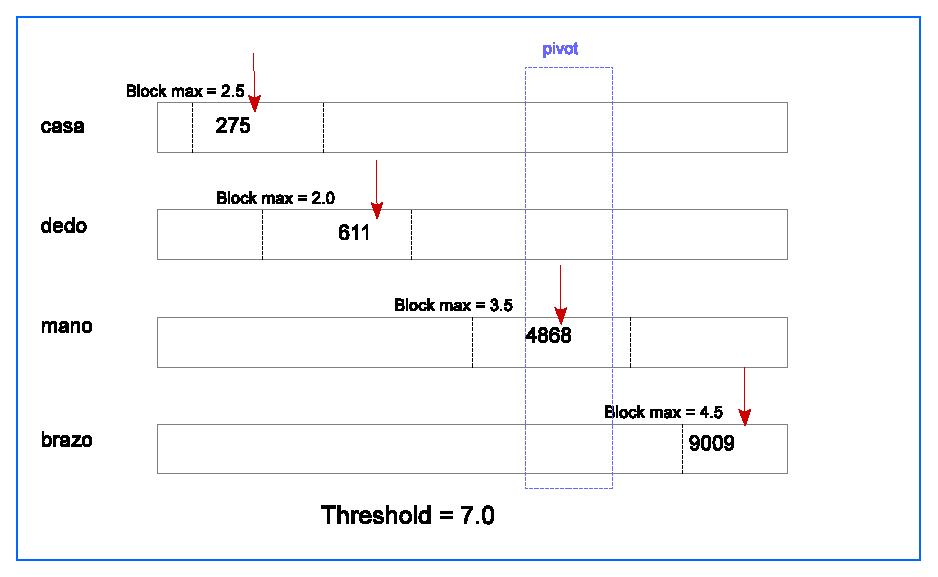
\includegraphics[scale=.75]{images/block-max-wand.eps}
\caption{Ejemplo del proceso \textit{Block-Max-Wand}}
\label{fig:bmw}
\end{figure}

\section{Predicción de tiempo de respuestas de transacciones de lecturas}
\label{marco:prediccion}
El rendimiento (\textit{performance}) de una consulta puede medirse de dos formas: Efectividad y eficiencia. La efectividad tiene relación con la calidad de los documentos extraídos para una cierta consulta y la eficiencia corresponde al tiempo que conlleva procesarla. El tiempo que le toma al sistema en resolver una consulta puede variar considerablemente. Con el objetivo de retornar los resultados al usuario dentro de una cota superior de tiempo, aquellas consultas que toman una mayor cantidad de tiempo en ser procesadas se requiere una mayor cantidad de procesadores para resolverla, de esta forma podemos asegurar esta cota de tiempo. El tener un buen predictor de la eficiencia de una transacción de lectura es muy útil, por ejemplo, si pensamos en un sistema con réplicas, podemos planificar la consulta en el servidor que se desocupará más pronto. 

Existen estudios en los cuales el rendimiento es inferido usando \textit{clarity score} \citep{Cronen-Townsend:2002}, que es una forma para evaluar la pérdida de ambigüedad de una transacción con respecto a la colección. En \citep{He:2004} se propone un conjunto de predictores para el rendimiento de cada consulta. Técnicas de aprendizaje de máquina también han sido estudiadas para predecir el rendimiento de transacciones de lectura \citep{Si:2002}. Todos los estudios mencionados anteriormente se han centrado en la efectividad para ser predicciones de rendimento de transacciones de lectura. La eficiencia de una transacción de lectura también ha sido objeto de estudio, identificando las principales razones que tienen impacto sobre el tiempo de respuesta y evaluando estos factores para predecir el comportamiento de futuras consultas \citep{Tonellotto:2011}. En \citep{Macdonald:2012} se propone un método de predicción de tiempo de respuesta para consultas basado en datos estadísticos disponibles en las respectivas listas invertidas de los términos. Finalmente, en \citep{Jeon:2014} además de utilizar estadísticos disponibles en las listas invertidas de los términos, se agregan estadísticos propios de las consultas para la creación de un predictor. 

\section{Scheduling en motores de búsqueda}
\label{marco:scheduling}
Los motores de búsqueda no solo se preocupan de la calidad de los resultados de las búsquedas (efectividad), sino que también de la velocidad con la que los resultados son obtenidos (eficiencia). Existen varias estrategias para mejorar la velocidad en la obtención de los resultados, una de ellas muy utilizada es el \textit{caching}. Consiste en guardar en memoria de acceso rápido (memoria caché) datos temporales, que luego pueden ser sobrescritos. Una opción es hacer \textit{caching} de los resultados de las búsquedas, de esta forma cuando una consulta es encontrada en caché el motor de búsqueda puede generar la respuesta rápidamente, reduciendo considerablementelos tiempos de calculos. Otra opción es, guardar en caché la intersección de las listas invertidas de pares comunes de términos que llegan al motor de búsqueda. Por ejemplo, si llega al sistema una consulta con los términos ('casa', 'árbol', 'perro'), se puede guardar en caché la intersección de las listas de 'casa' y 'árbol', para luego reutilizar esta información en otras consultas que lleguen en el futuro. Para ver más técnicas de \textit{caching} y ver el detalle de las técnicas mencionadas, ver \citep{Buttcher:2010}. 

Otra estrategia para acelerar el proceso de resolución de transacciones de lectura que llegan al sistema es el uso de algoritmos de planificación (scheduling). Un algoritmo de \textit{scheduling} es el proceso en el cual se cambia el orden en que llegan las consultas al motor de búsqueda con el objetivo de mejorar la eficiencia. 

Existen dos clases de algoritmos de \textit{scheduling}: estáticos y dinámicos. Los estáticos son aquellos en que se conoce el conjunto completo de tareas y las características de cada una de ellas, como por ejemplo, el tiempo de procesamiento. Los algoritmos de \textit{scheduling} dinámicos son aquellos en que no se conoce las tareas que llegarán en el futuro, también se desconoce el momento en que éstas llegarán. La filosofía de los algoritmos de \textit{scheduling} dinámicos es ajustarse a los cambios que pueden haber en el sistema.

En el contexto del presente trabajo de tesis, el objetivo de hacer \textit{scheduling} es minimizar el tiempo en que las consultas son procesadas por un motor de búsqueda. Los motores de búsqueda como \textit{Google}\footnote{http://www.google.com} o \textit{Yahoo!}\footnote{http://www.yahoo.com} trabajan en un contexto \textit{online}. Esto significa que cuando las consultas llegan al sistema (una a una), éste está obligado a tomar una decisión para planificarla sin saber cuáles transacciones de lectura llegarán en un momento posterior. A esto se le conoce como algoritmo de \textit{scheduling online} \citep{Albers:2003, Borodin:1998}.

Los sistemas de recuperación de información a gran escala despliegan una arquitectura distribuída \citep{Dean:2009}, en donde el índice invertido está particionado \citep{Barroso:2003} a lo largo de servidores (\textit{shard servers}), los cuales están encargados de procesar las transacciones de lectura que llegan al sistema. Es fácil notar que resolver una consulta con varios \textit{shard servers} mejoraría la eficiencia. Ahora bien, para asegurar un alto rendimiento (\textit{throughput}) del sistema, cada uno de los \textit{shard servers} poseen réplicas, de esta forma, más consultas pueden ser procesadas en paralelo en copias idénticas del mismo \textit{shard server}. Esto implica que el tiempo de espera de las transacciones de lectura que vienen llegando al sistema se reduce. 

En un sistema con arquitectura como el de la Figura \ref{fig:sistemaIR}, una transacción de lectura puede ser procesada por varios \textit{shard servers}, el \textit{broker} debe escoger la réplica más apropiada para procesar la parte de la consulta asignada al \textit{shard server}, con el objetivo de reducir el tiempo de espera de ésta. El \textit{broker} podría seleccionar el \textit{shard server} con el menor número de consultas en la cola, sin embargo, este no es un parámetro adecuado, ya que el tiempo de respuesta de las transacciones de lectura puede variar considerablemente, especialmente si se usa poda dinámica \citep{Broder:2003, Moffat:1996}. 

\begin{figure}[tp]
\centering
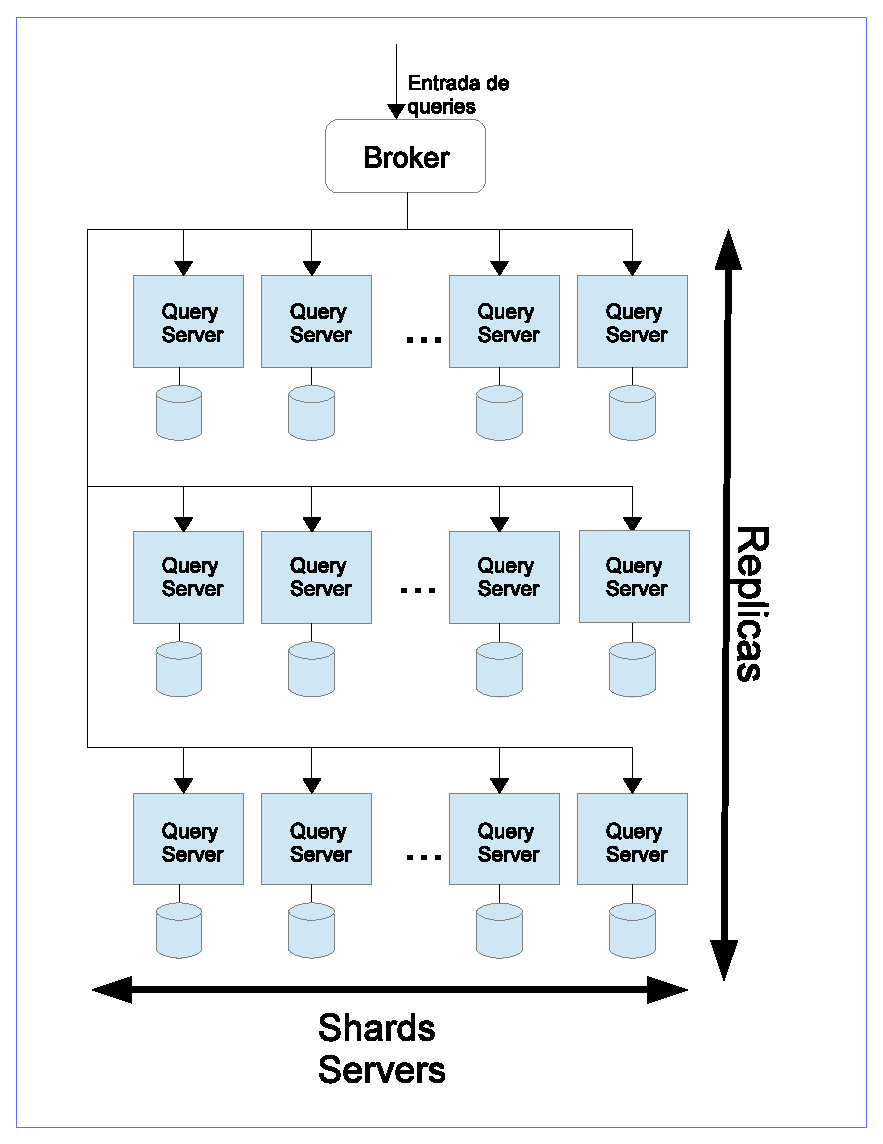
\includegraphics[scale=.75]{images/sistemaIR.eps}
\caption{Arquitectura de un sistema de recuperación de la información con réplicas}
\label{fig:sistemaIR}
\end{figure}

\subsection{Trabajo relacionado}
\label{marco:tr}
El estudio \citep{Broccolo:2013} analiza métodos de \textit{dropping} y \textit{stopping} para el procesamiento de consultas bajo altas carga de trabajo en un sistema distribuído donde existen múltiples servidores en el que cada uno resuelve una parte de la consulta para luego enviar las consultas al \textit{broker} y éste hace el \textit{merge} de los resultados de acuerdo al \textit{score} de los documentos. Se define un tiempo \textit{T}, en el que la suma de el tiempo de espera de la consulta para ser procesada ($t_{w}$) y el tiempo de procesamiento de la misma ($t_{p}$) deben ser menor a \textit{T}. Si es que se sobrepasa este tiempo, se tienen dos opciones (1) la consulta es desechada y se envía al \textit{broker} una lista vacía, (2) se detiene el procesamiento de la transacción de lectura y se envía los resultados parciales hasta el momento. Finalmente se propone un método basado en la predicción de tiempo de respuesta ($\hat{pt}(q)$) de una consulta \citep{Macdonald:2012} de modo que si se cumple $ \hat{pt}(q) \leq T - wt(q) $, entonces la consuta es desechada antes de comenzar a procesarse y se toma la siguiente desde la cola de espera. Notar que en estos métodos existe una pérdida de efectividad, puesto que eventualmente los servidores muchas veces no enviarán sus mejores documentos al \textit{broker}, esto implica que el \textit{broker} responderá al usuario un conjunto de K documento que no necesariamente son los mejores dentro del corpus completo.

En \citep{Freire:2012} se estudia el impacto que tiene la técnica de predicción de tiempos de respuestas para consultas, \citep{Tonellotto:2011} en sistemas de recuperación de la información con réplicas. En este estudio, se llega a la conclusión que usando una buena predicción, se puede reducir el tiempo que la consulta tiene que esperar para ser procesada ($t_{w}$), y también se puede reducir el tiempo total requerido para procesar el conjunto (\textit{log}) completo de transacciones de lectura (\textit{completion time}). En \citep{Freire:2013}, se propone un modelo híbrido de \textit{scheduling} de consultas a través de réplicas, en el que cuando el sistema se encuentre bajo altas cargas de trabajo, se utilice política de \textit{scheduling} basada en la predicción de tiempo de respuesta de las consultas \citep{Macdonald:2012} y cuando el sistema se encuentre con una baja carga de trabajo, se utilice una politica de \textit{scheduling} sencilla y de menor costo como \textit{Round Robin}.
\chapter{Estrategias de planificación de queries}
\label{cap:epq}


\section{Predicción del tiempo de respuesta a \textit{queries} en un motor de búsqueda}
\label{scheduling:ptrq}
Conocer de antemano la eficiencia de una \textit{query} es una ventaja importante para usar técnicas efectivas de \textit{scheduling} de \textit{queries} en motores de búsqueda. Existen estudios en los cuales la eficiencia es inferida usando \textit{clarity score} \citep{Cronen-Townsend:2002}, que es una forma para evaluar la pérdida de ambigüedad de una query con respecto a la colección. En \citep{He:2004} se propone un conjunto de predictores para la eficiencia de cada \textit{query}. Técnicas de aprendizaje de máquina también han sido estudiadas para predecir la eficiencia de \textit{queries} \citep{Si:2002}. Todos los estudios mencionados anteriormente se han centrado en la efectividad para ser predicciones. La eficiencia también ha sido utilizada para predecir el tiempo de respuesta de una query, identificando las razones por las que ésta puede ser resuelta ineficientemente y evaluando estos factores para predecir el comportamiento de futuras queries \citep{Tonellotto:2011}.

En el predictor propuesto en \citep{Macdonald:2012} está basado en estadísticos  disponibles de los términos de la query. 

\begin{tabular}{|l|}
\hline 
Estadístico del término s(t) \\ 
\hline 
1. Media aritmética del score \\ 
\hline 
2. Media geométrica del score \\ 
\hline 
3. Media armonica del score \\ 
\hline 
4. Puntaje máximo \\ 
\hline 
5. Varianza de puntaje \\ 
\hline 
6.  \\ 
\hline 
Agregadores \\ 
\hline 
Máximo \\ 
\hline 
Varianza \\ 
\hline 
Suma \\ 
\hline 
\end{tabular} 


Este predictor está evaluado comparado con 10.000 queries == individual and combinated


\section{Wand \textit{multi-threaded}}
\label{scheduling:wm}
Dado que el método WAND \citep{Broder:2003} consiste en el método del estado del arte ocupado hoy en día por los motores de búsqueda, en esta investigación se asume un sistema que usa este método para obtener eficientemente los mejores K documentos a una transacción de lectura. Este algoritmo usa un \textit{ranking} basado en una evaluación de dos niveles. En el primer nivel, este usa una cota superior (\textit{upper bound}) al puntaje de cada documento para intentar descartarlos eficientemente. En el segundo nivel se computa el puntaje real de los documentos que pasa el primer nivel. Para hacer que este proceso trabaje eficientemente, se usa una estructura de datos llamada \textit{heap} que va guardando el conjunto de los mejores K documentos hasta determinado instante. El menor puntaje de este conjunto es usado como umbral para las evaluaciones del primer nivel, de esta forma se descarta rápidamente documentos que no pueden ser parte del conjunto final de los \textit{top-K} documentos. Esto permite un eficiente y a la vez seguro proceso de descarte que asegura que en el resultado final se encontrará el conjunto correcto y no se perderán documentos relevantes.

Existen dos formas de implementar WAND \textit{multithreaded}. Uno de ellos es usando \textit{heaps} locales (LH), es decir, un \textit{heap} por \textit{thread} y el otro es usando \textit{heaps} compartidos (SH). El estudio en \citep{Rojas:2013} se muestra indicios que el esquema SH es generalmente más eficiente. Logrando rápidamente un óptimo valor para el threshold, el esquema SH posee las siguientes ventajas: (1) Se puede reducir el número de calculo de puntajes completjos y (2) son ejecutadas pocas operaciones de actualización del heap (reduciendo el número de locks que se hace a la estructura de dato). A continuación se presenta el diseño llevado a cabo para ambos esquemas.


\subsection{Wand con heaps locales}
\label{scheduling:whl}
En el esquema LH, cada thread procesa una porción del índice invertido mientras mantiene un heap local con los mejores K documentos que el específico thread ha encontrado hasta ahora. Al final del proceso, el resultado de cada thread debe ser reunido en un solo conjunto final global. Los resultados en \citep{Rojas:2013} muestran que el esquema LH es más eficientes para aquellas transacciones que toman poco tiempo en ser resueltas. En la Figura \ref{fig:wand-heap-local} se muestra el esquema de ejecución para heaps locales explicado anteriormente. 

\begin{figure}[tp]
\centering
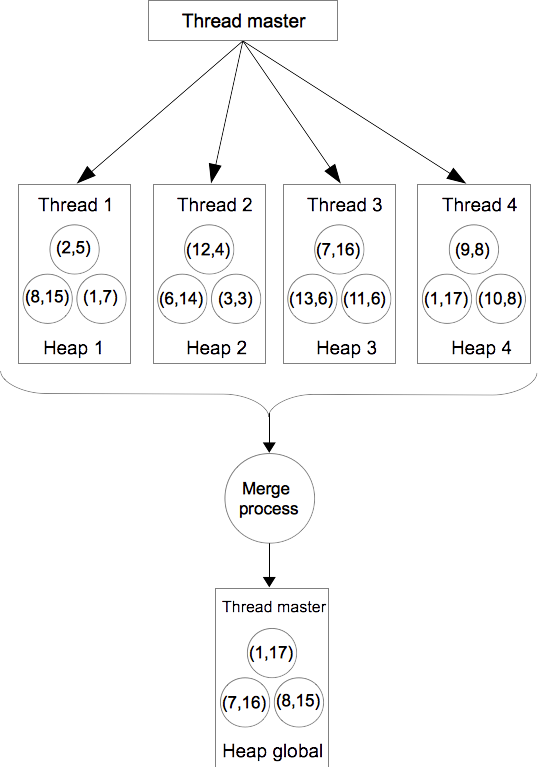
\includegraphics[scale=.75]{images/wand-heap-local.png}
\caption{Esquema de ejecución de algoritmo WAND con heaps locales}
\label{fig:wand-heap-local}
\end{figure}

El diseño aplicado para implementar el esquema LH se puede ver en la Figura \ref{fig:TopKMultiThreadWandOperatorLocal}. La clase principal es la TopKMultiThreadWandOperatorLocal, que es la encargada de controlar el paralelismo en la resolución de las transacciones. Para explicar de mejor manera cada una de las clases involucradas en la implementación, se presenta el siguiente diccionario de datos.

\begin{list}{}{}
	\item \textbf{TopKMultiThreadWandOperatorLocal}. Clase encargada de devolver los mejores K documentos para una query dada. Si es que la query debe ser resuelta en forma paralela, esta clase además debe controlar el paralelismo que se produce en la resolución de ésta, inicializando las variables correspondientes para lanzar los hilos de ejecución y luego escogiendo los mejores documentos desde todos los heaps creados por los diferentes threads (proceso de merge). En esta clase se define un mapa que asocia cada término del índice invertido con el puntaje del mejor documento en esa lista invertida (upper bound de la lista invertida) y además se define cuántos documentos se van a retornar al final del proceso (atributo K). El método execute inicializa las variables locales para los diferentes threads, posteriormente hace el llamado al método thread_execute (en el cual se llevará a cabo la resolución de la transacción de lectura en forma paralela), finalmente se toman los resultados parciales de cada uno de los hilos de ejecución y se ejecuta el proceso que mezcla los resultados, retornando solo los mejores K documentos. 
	
	\item \textbf{PartitionedInvertedIndex}. Clase que tiene la tarea de almacenar el índice invertido y extraer desde aquí las listas invertidas de documentos para cada uno de los términos de las transacciones de lectura. El almacenamiento el índice se lleva a cabo mediante un mapa cada término su lista invertida correspondiente y para la extracción de estas listas se usa el método getList.
	
	
	\item \textbf{TopKWandOperator}.  Cada thread tendrá su propio objeto TopKWandOperator encargado de obtener los mejores K documentos. El cálculo de este conjunto se realiza en el método execute con la ayuda de un objeto de tipo Wand asociado.
	
	\item \textbf{Wand}. Clase que controla la lógica del algoritmo wand. Lleva a cabo el proceso de inserción de documentos en el heap y todo lo que esto conlleva. 
	
	\item \textbf{ResultObject}. Clase que se utiliza para guardar los mejores K documentos.
	
	\item \textbf{QueryObject}. Clase que representa una transacción de lectura. Está constutuída sus términos,  las respectivas listas invertidas y pesos de cada uno de ellos, la cantidad de threads con los cuales se resolverá dicha transacción y el tiempo estimado de procesamiento (este tiempo se predice al momento de resolver la query).

\begin{figure}[H]
\centering
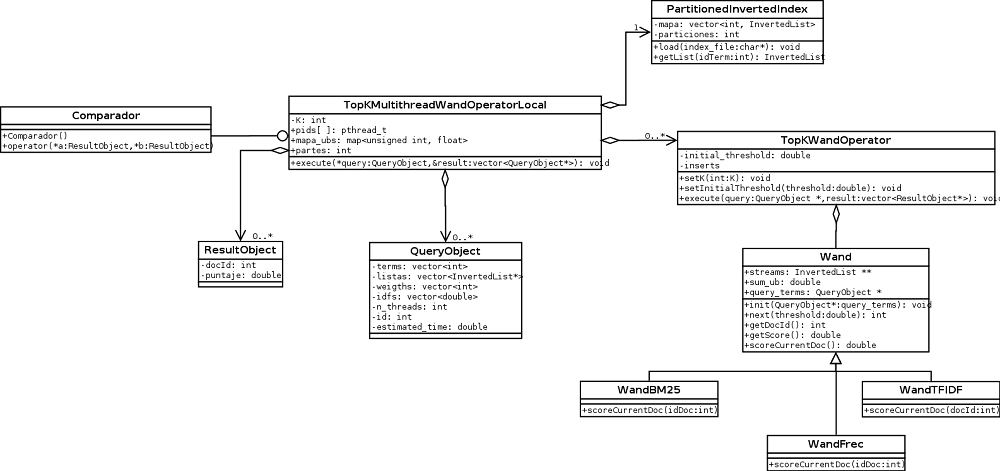
\includegraphics[scale=.75]{images/TopKMultiThreadWandOperatorLocal.png}
\caption{Diagrama de clases para el esquema LH}
\label{fig:TopKMultiThreadWandOperatorLocal}
\end{figure}


\subsection{Wand con heap compartido}
\label{scheduling:whc}
En el esquema SH cada thread procesa una perción del índice. Sin embargo, un solo heap es creado y accedido por todos los threads. En este caso no se requiere de mezcla y el proceso de descarte tiende a ser más eficiente porque los documentos con mayor puntaje tienden a estar en el heap. Sin embargo acceder al heap debe ser controlado por un lock o algún método similar que garantice el acceso exclusivo de los threads al heap.

\begin{figure}[H]
\centering
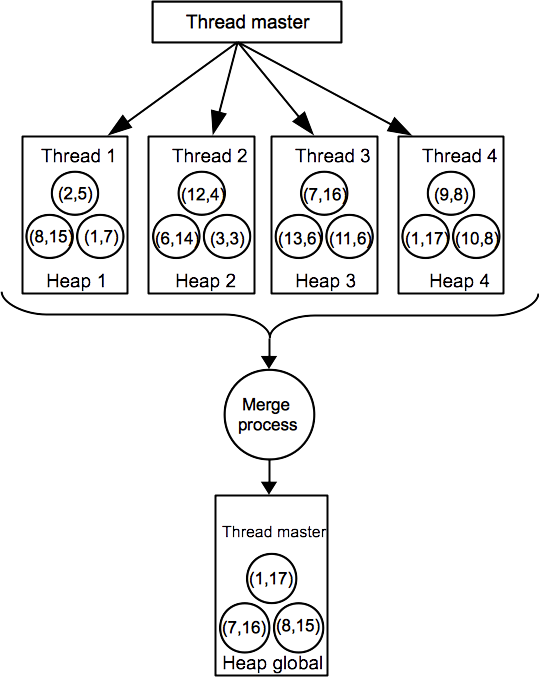
\includegraphics[scale=.75]{images/wand-heap-compartido.png}
\caption{Esquema de ejecución de algoritmo WAND con heap compartido}
\label{fig:wand-heap-compartido}
\end{figure}

\begin{figure}[H]
\centering
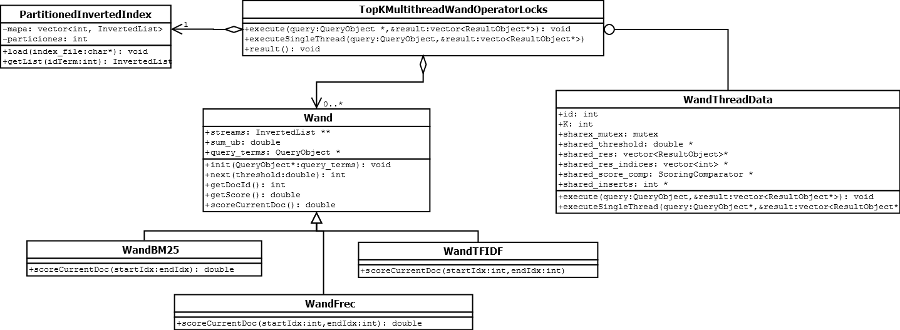
\includegraphics[scale=.75]{images/TopKMultiThreadWandOperatorLocks.png}
\caption{Diagrama de clases para el esquema SH}
\label{fig:TopKMultiThreadWandOperatorLocks}
\end{figure}






\section{Estrategia \textit{baseline}}
\label{scheduling:baseline}
Una simple manera de construir un sistema que responda a múltiple queries simultáneamente usando múltiple threads es, usando los threads de manera independiente. Para hacer esto, se debe mantener un conjunto de threads consumidores, cada uno de ellos se encargará de responder a queries secuencialmente y todos ellos trabajan en paralelo leyendo las queries desde la misma cola. Esto es lo que en este trabajo se denomina Un Thread Por Query (1TQ), ver Figura X (Profundizar más en esta figura)

Este esquema simple tiene ventajas y desventajas, además que es fácil de implementar y controlar. 

Existen sistemas que tienen que ejecutar un conjunto de queries de un cierto tamaño y luego parar para actualizar la información del índice invertido. Solo después de la fase de actualización, éste es capaz de ejecutar el siguiente conjunto de queries (batch de queries). Al final de cada batch, es posible que algunos threads finalicen su trabajo y que no tengan más queries para procesar, por lo que ellos tienen que esperar que los threads restantes finalicen su trabajo antes que el sistema entre en la fase de actualización. 

Sin embargo, aunque cada thread está secuencialmente ejecutando una query diferente, algunas de estas operaciones puede tomar un tiempo cosiderable, de esta forma se produce una importante pérdide de eficiencia, aunque la intuición nos dice que esto se puede amortizar con trabajos pequeños. Ver Figura 2 (Explicar)




\section{Estrategias de \textit{scheuling}}
\label{scheduling:es}
nosotros optamos por un enfoque de Wand Heap Compartido para ser usado en los experimentos.
\subsection{FR}
\label{scheduling:fr}

\subsection{Times}
\label{scheduling:times}

\subsection{TimesRanges}
\label{scheduling:timesranges}




\section{Estrategia de unidades de trabajo}
\label{scheduling:unidadestrabajo}
%\chapter{Wand \textit{multi-threaded}}
\label{cap:wand}
Dado que el método Wand \citep{Broder:2003} consiste en el método del estado del arte ocupado hoy en día por los motores de búsqueda para obtener eficientemente los mejores K documentos, en este trabajo se utiliza un sistema que trabaja con este método. Este algoritmo usa un \textit{ranking} basado en una evaluación de dos niveles. En el primer nivel, usa una cota superior (\textit{upper bound}) al puntaje de cada documento para intentar descartarlos eficientemente. En el segundo nivel se computa el puntaje real de los documentos que pasa el primer nivel. Se utiliza una estructura de datos llamada \textit{heap} que va guardando el conjunto de los mejores $K$ documentos hasta un determinado instante. El menor puntaje de este conjunto es usado como umbral (\textit{threshold}) para las evaluaciones del primer nivel, de esta forma se descarta rápidamente documentos que no pueden ser parte del conjunto final de los \textit{top-K} documentos. Esto permite un eficiente y a la vez seguro proceso de descarte que asegura que en el resultado final se encontrará el conjunto correcto y no se perderán documentos relevantes.

Existe una variación al método Wand tradicional que intenta hacer una poda más agresiva, en otras palabras, lo que se intenta es tratar de omitir una mayor cantidad de documentos a la hora de resolver una transacción de lectura. Este método llamado Block Max Wand requiere que cada una de las listas invertidas este particionada en bloques (generalmente 64 o 128 bloques), en donde se tiene un upper bound por cada bloque. La lógica es la misma que en el método original y en la primera fase también se ocupa el máximo puntaje por lista para descartar documento, sin embargo, ahora existe una tercera fase en donde se utiliza el upper bound por bloques. De esta forma se intenta omitir una mayor cantidad de documentos. Más detalle de estos métodos se pueden encontrar en las secciones \ref{marco:wand} y \ref{marco:bmw}.

Wand y Block Max Wand son métodos lógicamente parecidos en el sentido que trabajan con \textit{upper bounds} para poder descartar documentos, es por esto que el diseño de la implementación es como lo muestra la Figura \ref{fig:diagramawand}; aquí se puede apreciar dos tipos de Wand: WandScorer y WandMaxBlock. WandScorer implementa el método tradicional utilizando el método \textit{next}, que retornará algún documento que merezca estar en el conjunto \textit{top-K} en ese momento. Por su parte, WandMaxBlock además de utilizar la función \textit{$next()$}, usa la función \textit{$nextShallow()$}, que moverá el puntero del documento actual de la lista a la posición inicial del bloque en donde debería encontrarse el documento que se le entrega como parámetro. 
La ventaja de este diseño es que ambas opciones son flexibles a utilizar cualquier función de \textit{ranking} que se desee, en el diagrama se observa que se utilizará BM25.

\begin{figure}[!th]
\centering
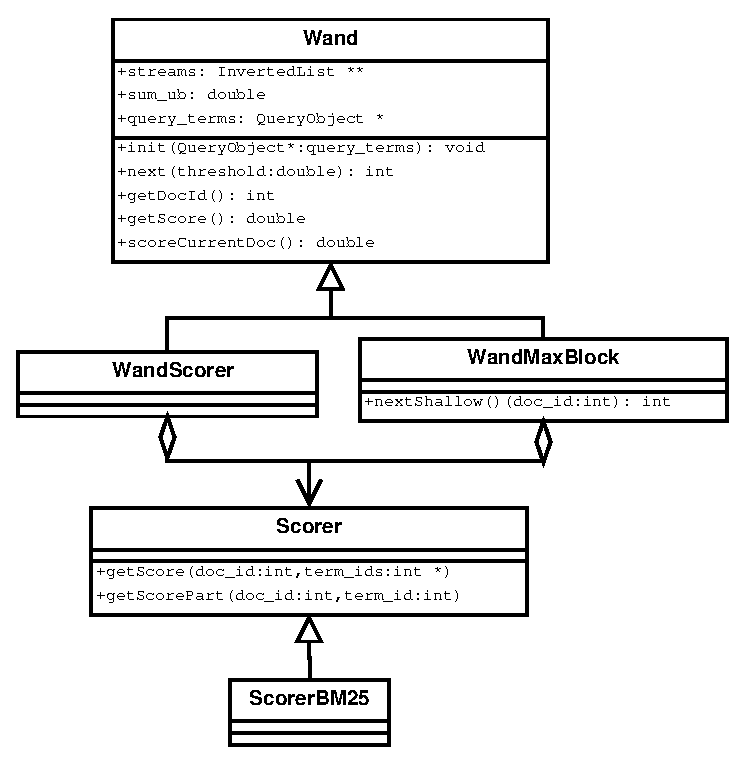
\includegraphics[scale=.75]{images/WAND.eps}
\caption{Diseño de clases para Wand y Block Max Wand.}
\label{fig:diagramawand}
\end{figure}

Existen dos formas de implementar Wand. Una de ellas es usando \textit{heaps} locales (LH), es decir, un \textit{heap} por hilo de ejecución y el otro es usando \textit{heaps} compartidos (SH). En el estudio \citep{Rojas:2013} se muestran indicios que el esquema SH es generalmente más eficiente, logrando rápidamente un óptimo valor para el \textit{threshold}. El esquema SH posee las siguientes ventajas: (1) Se puede reducir el número de cálculos de puntajes completos y (2) se ejecutan pocas operaciones de actualización del \textit{heap} (reduciendo el número de \textit{locks} que se hace a la estructura de dato). 
A continuación se muestra las dos formas en que se implementó Wand y también la implementación de Block Max Wand.


\section{Wand con \textit{heaps} locales}
\label{scheduling:wlh}
En el esquema LH, cada hebra procesa una parte del índice invertido mientras mantiene un \textit{heap} local con los mejores $K$ documentos. Al finalizar este proceso, los resultados se unen en un solo conjunto final global. Los resultados en \citep{Rojas:2013} muestran que el esquema LH es más eficiente para aquellas transacciones que toman poco tiempo en ser resueltas. En la Figura \ref{fig:wand-heap-local} se muestra el esquema de ejecución para \textit{heaps} locales explicado anteriormente. 

\begin{figure}[!ht]
\centering
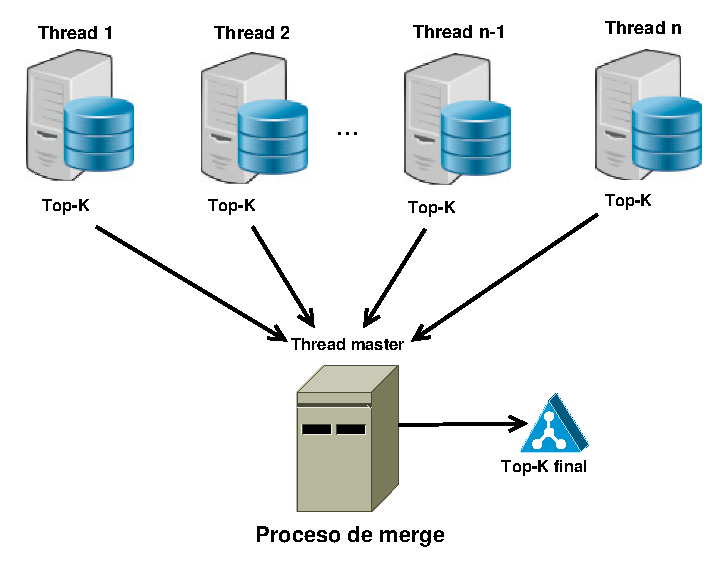
\includegraphics[scale=.75]{images/wand_heaps_locales.eps}
\caption{Esquema de ejecución de algoritmo WAND con \textit{heaps} locales.}
\label{fig:wand-heap-local}
\end{figure}

El diseño aplicado para implementar el esquema LH se puede ver en la Figura \ref{fig:TopKMultiThreadWandOperatorLocal}. La clase principal es la TopKMultiThreadWandOperatorLocal, que es la encargada de controlar el paralelismo en la resolución de las transacciones. Para explicar de mejor manera cada una de las clases involucradas en la implementación, se presenta el siguiente diccionario de datos.

\begin{figure}[!ht]
\centering
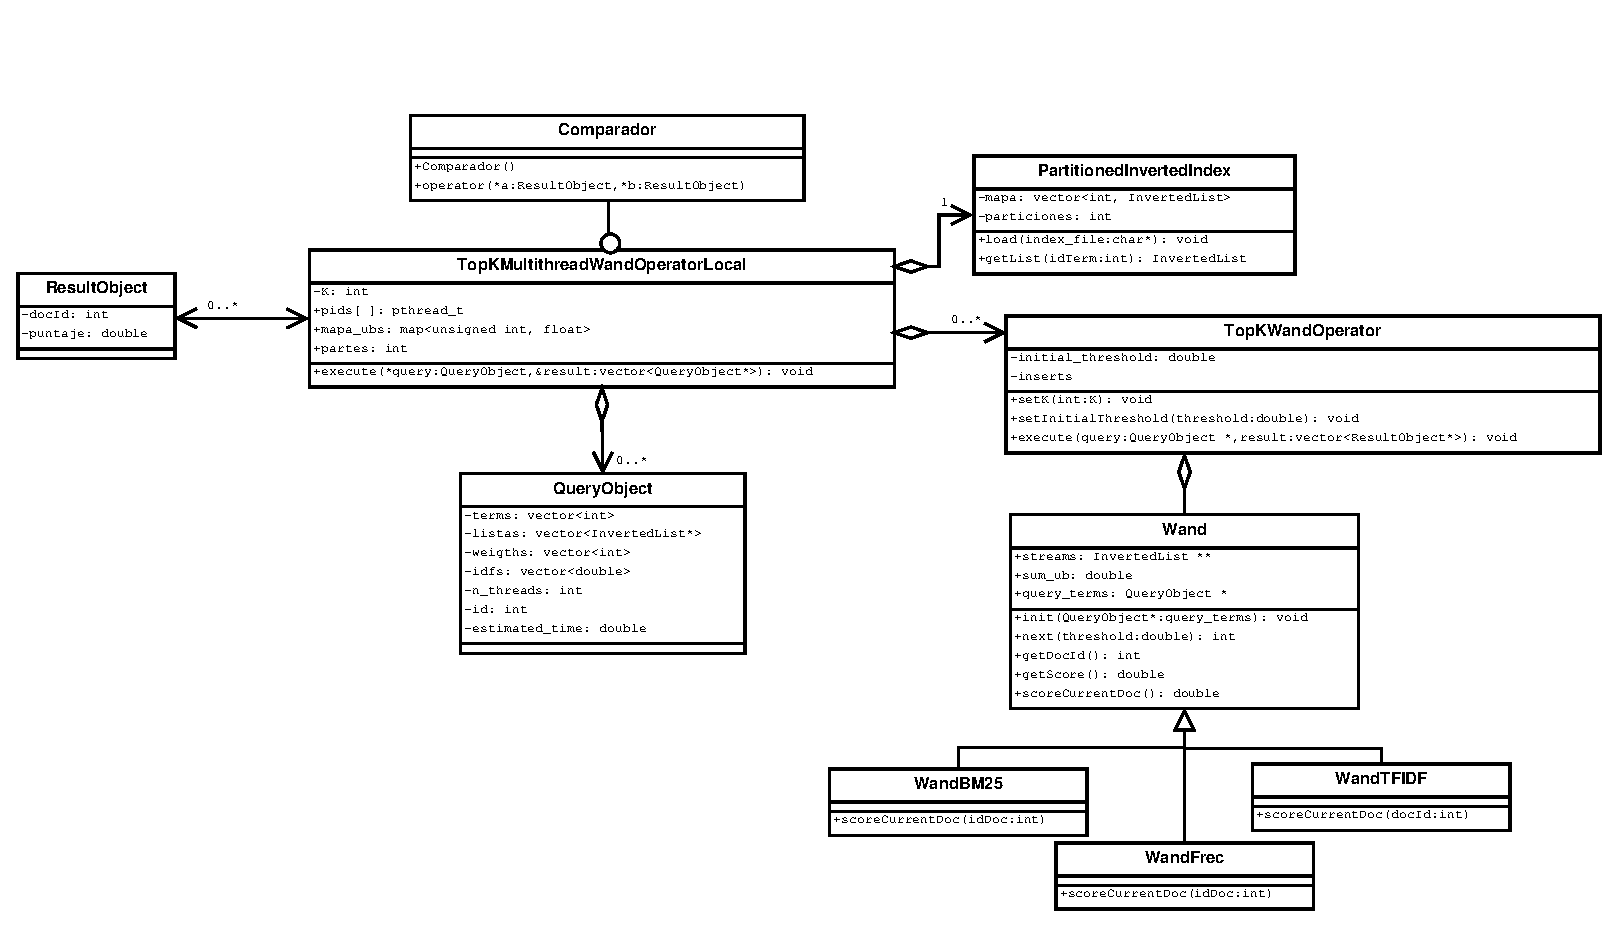
\includegraphics[scale=.75]{images/TopKMultiThreadWandOperatorLocal.eps}
\caption{Diagrama de clases para el esquema LH.}
\label{fig:TopKMultiThreadWandOperatorLocal}
\end{figure}

\begin{list}{}{}
	\item \textbf{TopKMultiThreadWandOperatorLocal}. Clase encargada de devolver los mejores $K$ documentos para una consulta dada. Si es que la consulta debe ser resuelta en forma paralela, esta clase además debe controlar el paralelismo que se produce en la resolución de ésta, inicializando las variables correspondientes para lanzar los hilos de ejecución y luego escogiendo los mejores documentos desde todos los \textit{heaps} creados por los diferentes hilos de ejecución (proceso de \textit{merge}). En esta clase se define un mapa que asocia cada término del índice invertido con el puntaje del mejor documento en esa lista invertida (upper bound de la lista invertida) y además se define cuántos documentos se van a retornar al final del proceso (atributo K). El método \textit{execute} inicializa las variables locales para las diferentes hebras, posteriormente hace el llamado al método \emph{thread-execute} (en el cual se llevará a cabo la resolución de la transacción de lectura en forma paralela), finalmente se toman los resultados parciales de cada uno de los hilos de ejecución y se ejecuta el proceso que mezcla los resultados, retornando solo los mejores $K$ documentos. 
	
	\item \textbf{PartitionedInvertedIndex}. Clase que tiene la tarea de almacenar el índice invertido y extraer desde aquí las listas invertidas de documentos para cada uno de los términos de las transacciones de lectura. El almacenamiento del índice se lleva a cabo mediante un mapa, en donde cada término tiene asociado su lista invertida correspondiente y para la extracción de estas listas se usa el método getList.
	
	\item \textbf{TopKWandOperator}.  Cada hilo tendrá su propio objeto TopKWandOperator encargado de obtener los mejores $K$ documentos. El cálculo de este conjunto se realiza en el método \textit{execute} con la ayuda de un objeto de tipo Wand asociado.
	
	\item \textbf{Wand}. Clase que controla la lógica del algoritmo wand. Lleva a cabo el proceso de inserción de documentos en el \textit{heap} y todo lo que esto conlleva. Existen diferentes tipos de objetos Wand que se pueden utilizar, entre ellos están WandBM25, WandFrec y WandTFIDF, donde la única diferencia entre ellos es el método con que se calcula el puntaje de cada documento. Por ejemplo, WandBM25 utiliza BM25 y WandTFIDF utiliza tf-idf. 
	
	\item \textbf{ResultObject}. Clase que se utiliza para guardar los mejores $K$ documentos.
	
	\item \textbf{QueryObject}. Clase que representa una transacción de lectura. Está formada por términos y sus respectivas listas invertidas, la cantidad de hebras con las cuales se resolverá dicha transacción y el tiempo estimado de procesamiento (este tiempo se predice al momento de resolver la consulta).

\end{list}


\section{Wand con \textit{heap} compartido}
\label{scheduling:whc}
En el esquema SH cada hebra procesa una parte del índice. Sin embargo, ahora un solo \textit{heap} es creado y accedido por todos los hilos de ejecución. En este caso no se requiere de mezclar los resultados y el proceso de descarte tiende a ser más eficiente porque los documentos con mayor puntaje tienden a estar en el \textit{heap}. El acceso al \textit{heap} debe ser controlado por un \textit{lock} o algún método similar que garantice el acceso exclusivo de los hilos al \textit{heap}. Este esquema es más eficiente que el LH en consultas que toman mayor tiempo en ser resueltas.

El diseño implementado para este esquema posee como clase principal a TopKMultiThreadWandOperatorLocks y difiere del modelo implementado para el esquema LH en el sentido que ahora se debe controlar el acceso concurrente a los datos compartidos como el \textit{heap} y el \textit{threshold}. A continuación se presenta el diccionario de datos del esquema SH mostrado en la Figura \ref{fig:TopKMultiThreadWandOperatorLocks}.

\begin{figure}[!ht]
\centering
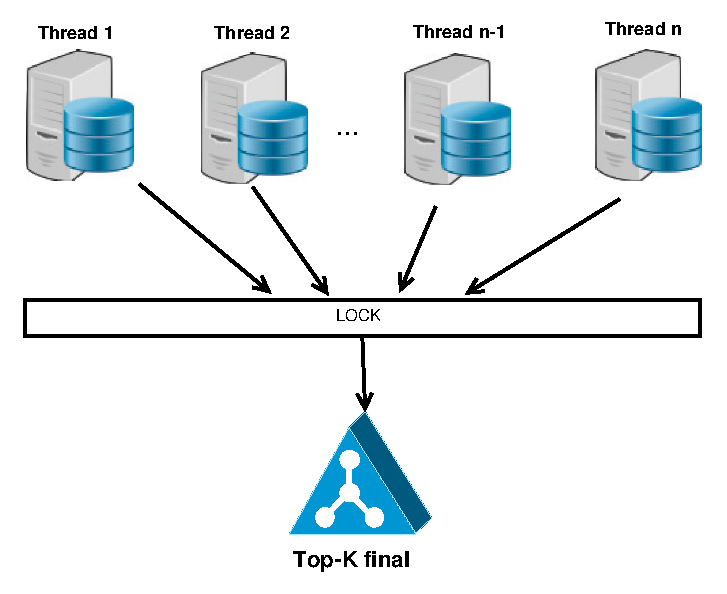
\includegraphics[scale=.75]{images/wand_heaps_compartido.eps}
\caption{Esquema de ejecución de algoritmo WAND con \textit{heap} compartido.}
\label{fig:wand-heap-compartido}
\end{figure}

\begin{list}{}{}
	\item \textbf{TopKMultiThreadWandOperatorLocks}. Clase encargada de inicializar las variables compartidas y de lanzar los hilos de ejecución requeridos para procesar la transacción de lectura.
	
	\item \textbf{WandThreadData}. Clase anidada a TopKMultiThreadWandOperatorLocks que contendrá todas las variables compartidas para el procesamiento de las consultas. Dentro de los atributos más importantes destaca el mutex utilizado para controlar el acceso al \textit{heap} compartido y además al \textit{threshold} (en este esquema es un \textit{threshold} global y compartido por todas las hebras).
	
	\item \textbf{Wand}. Al igual que en el esquema anterior, esta clase se encarga de llevar a cabo el proceso de inserción de documentos en el \textit{heap} y de las actualizaciones del \textit{threshold}. El método \textit{scoreCurrentDoc} es el encargado de entregarle un puntaje a cada documento y dependerá de qué tipo de Wand se este utilizando (BM25, WandFrec, WandTFIDF). 

	\item \textbf{PartitionedInvertedIndex}. Clase encargada de almacenar el índice invertido. Posee un método llamado getList que recibe como parámetro el identificador de un documento y retorna la lista invertida asociada. 

\end{list}

\begin{figure}[!ht]
\centering
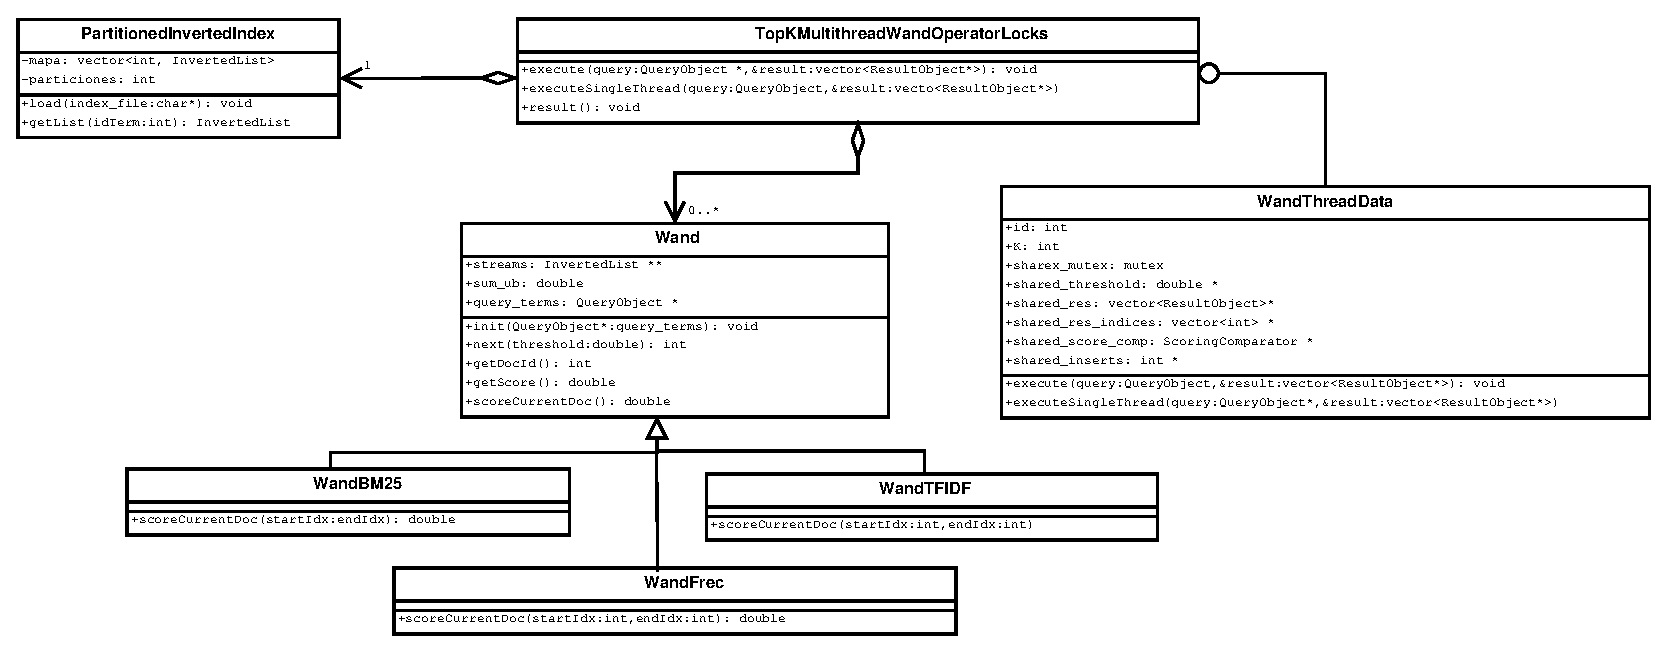
\includegraphics[scale=.75]{images/TopKMultiThreadWandOperatorLocks.eps}
\caption{Diagrama de clases para el esquema SH.}
\label{fig:TopKMultiThreadWandOperatorLocks}
\end{figure}

\section{Block max wand}
Recordar que en el método de Wand para descartar documentos y encontrar un documento que potencialmente podría estar en el conjunto \textit{top-K}, utiliza los \textit{upper bounds} globales de cada lista, es decir, la máxima contribución (puntaje o \textit{score}) de algún documento de la lista invertida. Además, Wand tradicional es una estrategia DAAT, por lo que por cada lista invertida ocupa un puntero al documento actual que se desea evaluar; también usa un método que recibe como entrada un identificador del documento $docID$ y una lista invertida $L$, y retorna el primer $docID'$ que sea mayor o igual al documento $docID$. A esto se le conoce como movimiento de puntero profundo (\textit{deep pointer movement}) debido a que generalmente implica una descompresión del bloque en el que se encuentra el documento.

Sin embargo, como se dijo anteriormente en \ref{marco:bmw}, usando solo las máximas contribuciones por cada bloque no hará que el método funcione correctamente, puesto que hará que eventualmente se pierdan documentos que podrían estar en el conjunto final de los mejores $K$ documentos. Como ahora se tiene las máximas contribuciones por cada bloque, BMW utiliza otra función la cual recibe como parámetro un identificador de documento $docID$ y una lista invertida. Lo que se hace es mover el puntero actual al correspondiente bloque donde eventualmente se debería encontrar el documento $docID$. A esta función se le conoce como movimiento de puntero superficial (\textit{shallow pointer movement}), por la razón que no involucra una descompresión de bloque. Se debe notar que para que esta función trabaje correctamente se requiere tener almacenada las fronteras de cada uno de los bloques de las listas invertidas.

BMW utiliza dos principales ideas en su diseño: (1) Se usa los \textit{upper bounds} globales para determinar un pivote candidato (como en Wand tradicional), para luego usar los \textit{upper bounds} locales para determinar si es que el pivote candidato es un pivote real o no, y (2) Se intenta siempre utilizar \textit{shallow pointer movement} por sobre \textit{deep pointer movement}.

En el Algoritmo \ref{alg:bmw} se puede apreciar cómo el método \textit{Block-Max-Wand} trabaja. Recordar que todas las listas invertidas poseen un puntero al documento actual que se desea evaluar (\textit{currentDoc}). Lo primero que se hace es ordenar de manera creciente las listas invertidas de acuerdo a su correspondiente \textit{currentDoc}. La función \textit{findPivot()} es la misma que se utiliza en el método Wand tradicional (\ref{marco:wand}), se itera sobre las listas invertidas y se retorna la posición de la lista en donde se cumple que la suma de los \textit{upper bounds} globales es mayor al \textit{threshold} ($\theta$). Luego la función \textit{$NextShallow()$} se encarga de avanzar los punteros de las listas invertidas al inicio del bloque que debería contener el documento $d$. Posteriormente la función \textit{isRealPivot()} verifica si es que el pivote $p$ encontrado es un pivote real o no, para cada una de las listas desde la posición $0$ hasta la posición $p$, se suma los \textit{upper bounds} de los bloques en donde se encuentran los punteros (recordar que con \textit{$NextShallow()$} los punteros de las listas quedaron apuntando a los bloques en donde se debería encontrar el documento $d$), si la suma es mayor al \textit{threshold} entonces retorna verdadero, de lo contrario retorna falso. El método \textit{scoreDoc()} calcula el puntaje del documento que se le pasa por parámetro. 

Cuando el método se da cuenta que $p$ no es un pivote real, lo que se hace es buscar un nuevo candidato a través de la función \textit{getNewCandidate()}, la cual hace avanzar los punteros de las listas invertidas hasta el bloque siguiente que contenga el mínimo $docID$. Para explicar de mejor manera esta idea se presenta la Figura \ref{fig:getNewCandidate}, aquí se puede ver que el documento $4868$ es el pivote, cuando este documento no es un pivote real (la función \textit{isRealPivote} retorna falso), lo que se hará es escoger un documento $d'$ tal que $d = min(d1,d2,d3,d4)$ en donde $d1,d2,d3$ son la frontera del bloque actual más uno (inicio del bloque siguiente) y $d4$ es el \textit{currentDoc} de la cuarta lista. Notar que para hacer un descarte seguro de documentos, siempre se debe incluir a la elección del nuevo candidato el \textit{currentDoc} de la lista inmediatamente siguiente a la lista pivote (en este caso 9009).  

\begin{figure}[!th]
\centering
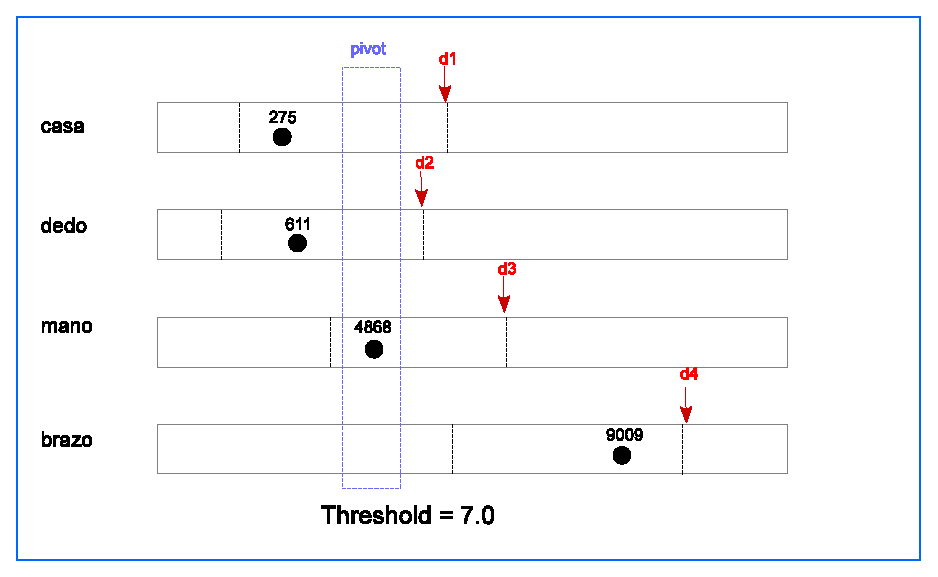
\includegraphics[scale=.75]{images/get_new_candidate.eps}
\caption{Ejemplo de cómo opera la functión getNewCandidate().}
\label{fig:getNewCandidate}
\end{figure}

\begin{algorithm}[!th]
\caption{\em $BMW(\theta, L, docID): Block Max Wand$}
\label{alg:bmw}
\begin{algorithmic}[1]
\REQUIRE Un \textit{threshold} $\theta$, listas invertidas $L$ de los términos en la consulta
\ENSURE $docID$, si existe un documento $docID$ tal que $score(docID)$ $\geq$ $\theta$. de lo contrario END-OF-FILE
\WHILE {true}
	\STATE $Sort(L);$
	\STATE $p = findPivot(L,\theta);$
	\STATE $d = L[p] \rightarrow currentDoc;$
	\IF {$d == $ END-OF-FILE}
  		\STATE $break;$
	\ENDIF
		
	\FOR {$ i = 0...p $}
		\STATE $NextShallow(d, L[i]);$
	\ENDFOR
	
	\IF {$isRealPivot(\theta, p);$}
		\IF {$L[0] \rightarrow currentDoc == d$}
			\STATE $scoreDoc(d, p);$
			\FOR {$ i = 0...p $}
				\STATE $Next(d + 1, L[i]);$
			\ENDFOR
		\ELSE
			\WHILE {$List[p - 1] \rightarrow currentDoc == p $}
				\STATE $p = p - 1;$			
			\ENDWHILE
			
			\FOR {$ i = 0...p $}
				\STATE $Next(d, L[i]);$
			\ENDFOR
			
		\ENDIF		
	\ELSE	
		\STATE $d' = getNewCandidate();$
		\FOR {$ i = 0...p $}
			\STATE $Next(d', L[i]);$
		\ENDFOR
	\ENDIF
	
\ENDWHILE

\end{algorithmic}
\end{algorithm}
%\chapter{Diseño e implementaci\'on de RBOX 2.0}
\label{cap:diseno}

En este capítulo se presenta el diseño e implementación de RBOX 2.0 una herramienta de software construida en \textit{Java} basada en el modelo de representación de datos propuesto en este trabajo de tesis.

El \textit{framework} esta construido en \textit{Java SE 7} por las siguientes razones:

\begin{itemize}
	\item \textbf{Popularidad}: según el \textit{ranking} presentado por \textbf{TIOBE}\footnote{http://www.tiobe.com/index.php/content/paperinfo/tpci/index.html} mensualmente \textit{Java} es el segundo lenguaje más popular, precedido sólo por C.  
	\item \textbf{Portabilidad}: las aplicaciones construidas en \textit{Java} son ejecutadas bajo su máquina virtual. Por lo tanto pueden ejecutarse en cualquier dispositivo físico que posea la máquina virtual.
	\item \textbf{Gran cantidad de librerías}: en \textit{Java} se proveen varias librerías que agilizan el desarrollo como por ejemplo \textit{Apache Commons}\footnote{http://commons.apache.org/},   \textit{fastutils}\footnote{http://fastutil.di.unimi.it/}, etc. En el caso de SR se proveen varias librerías de minería de datos y aprendizaje de máquina tales como: \textit{Weka}\footnote{http://www.cs.waikato.ac.nz/ml/weka/}, \textit{Apache Mahout}\footnote{http://mahout.apache.org/}, \textit{Mallet}\footnote{http://mallet.cs.umass.edu/} entre otras.
	\item \textbf{Integración con ambientes empresariales}: la versión empresarial \textit{Java EE 6}\footnote{http://www.oracle.com/technetwork/java/javaee/overview/index.html} provee un estándar para la construcción de aplicaciones empresariales.
\end{itemize}


\section{Arquitectura de RBOX 2.0}

% % Arquitectura propuesta para RBOX 2.0

RBOX\footnote{Acrónimo de \textbf{R}ecommendation \textbf{BOX} } 2.0 es una herramienta para el diseño e implementación de SR basados en el modelo de representación de datos propuesto que permite que los SR tengan la capacidad de situar los eventos.

En la Figura \ref{fig:arquitectura} se muestra la arquitectura de RBOX 2.0 donde se observan los principales componentes de la herramienta.

\begin{itemize}
\item \textbf{Representación de datos}: se compone de dos componentes que representan los contenedores de sentido y la lógica de la \textit{3-Ontology}.
\item \textbf{Algoritmos de recomendación}: pueden estar construidos con herramientas de construcción de SR de filtrado colaborativo como \textit{Lenskit} o de minería de datos como \textit{Weka}.
\item \textbf{RBOX Recommender}: corresponden a los componentes que permiten dar el servicio de recomendación.
\end{itemize}


\begin{figure}[tp]
	\centering
	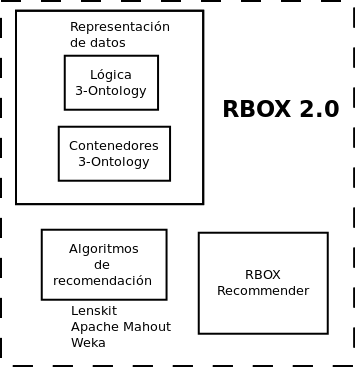
\includegraphics[scale=.6]{images/arquitectura.png}
	\caption{Arquitectura RBOX 2.0 }
	\label{fig:arquitectura}
\end{figure}

RBOX 2.0 se compone de los módulos API y CORE el primero establece la definición de las interfaces y el segundo una implementación para la construcción de SR. En la Figura \ref{fig:diagramapaquetes} se presenta un diagrama de paquetes de RBOX 2.0 con sus dos módulos principales y sub-módulos.

\begin{figure}[tp]
	\centering
	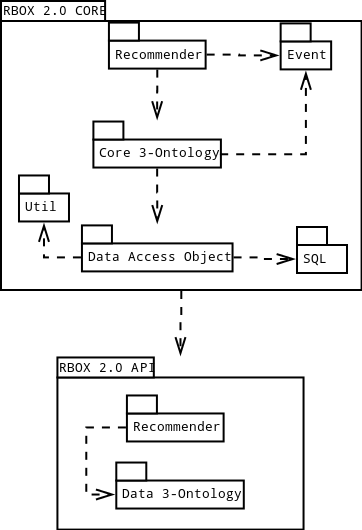
\includegraphics[scale=.6]{images/arquitectureRBOX2.png}
	\caption{Diagrama de paquetes de RBOX 2.0 }
	\label{fig:diagramapaquetes}
\end{figure}

\subsection{RBOX 2.0 API}

Corresponde a la definición de las interfaces  que permiten la representación de datos \textit{(data 3-ontology)} y construcción de  \textit{(recommender)}. Este módulo se compone de los siguientes sub-módulos:

\begin{itemize}
	\item \textbf{Recommender}: corresponde a la definición de las interfaces que permiten construir un recomendador.
	\item \textbf{Data 3-Ontology}: corresponde a la definición de las interfaces que representan los contenedores de sentido y la lógica de la \textit{3-Ontology}.
\end{itemize}

\subsection{RBOX 2.0 CORE}

Corresponde a una implementación del API y un conjunto de módulos que permiten construir un SR. Este módulo se compone de los siguientes sub-módulos:

\begin{itemize}
	\item \textbf{Recommender}: provee una implementación de las interfaces de recomendación.
	\item \textbf{Event}: implementación de componentes para la representación de distintos tipos de eventos.
	\item \textbf{Core 3-Ontology}: componentes que describen el comportamiento del \textit{framework 3-ontology}.
	\item \textbf{Utils}:  componentes utilitarios como por ejemplo de lectura de archivos. 
	\item \textbf{Data access object}: definición e implementación de los componentes DAO definidos.
	\item \textbf{SQL}: definición e implementación de componentes para el acceso a base de datos relacionales mediante JDBC.
	\end{itemize}

\section{Diseño de clases de RBOX 2.0}

En esta sección se realiza la definición de las clases utilizadas que representan el modelo propuesto en el capítulo \ref{capitulo:modelo}.

\subsection{Contenedores de sentido}

La \textit{3-ontology} define tres contenedores de sentido eventos, comunidades y lugares. Cada uno de estos conceptos es representado mediante una interfaz para proveer la flexibilidad y extensibilidad requerida por los SR. Por otro lado, se presentan las representaciones de dos conceptos básicos para un SR como son el usuario e ítem.

En el código \ref{cod:event} se presenta la definición de la  interfaz que representa a un evento que puede ser extendida a nuevos tipos de eventos dado que el valor es de tipo genérico. Se proveen implementaciones para dos eventos interactivos y sociales:

\begin{itemize}
	\item \textbf{Rating}: en este caso el valor es de tipo real bajo un dominio determinado.
	\item \textbf{Tagging}: en este caso el valor es una cadena de caracteres (\textit{String}).
\end{itemize}


\begin{lstlisting}[float, caption = Interfaz Event, label = cod:event]
public interface Event {

   long getUserId();

   long getItemId();

   long getTimestamp();
dos
   long getPlaceId();

   long getCommunityId();  

   <T> T getValue();
}
\end{lstlisting}

 En el código \ref{cod:community} se muestra la definición de la interfaz que representa a una comunidad. Esta hereda de \textit{List} y se compone de usuarios. Un usuario puede explícitamente indicar su pertenencia a una comunidad implícitamente o se puede deducir dado su perfil e historial de eventos. 

\begin{lstlisting}[float, caption = Interfaz Community, label = cod:community]
public interface Community extends List<User>{  

    long getId();

    String getName();
   
    LongSet getUserIds();
}
\end{lstlisting}

En el código \ref{cod:place} se muestra la definición de la interfaz que representa a un lugar. Esta hereda de \textit{List} y se compone de ítems. Un lugar corresponde al espacio físico y/o virtual donde habitan los ítems y son realizados los eventos. 

\begin{lstlisting}[float,caption = Interfaz Place, label = cod:place]
public interface Place extends List<Item> {   

    long getId();
  
    String getName();

    LongSet getItemIds();  
}
\end{lstlisting}

Un usuario es el protagonista de un evento, pertenece a una o varias comunidades. La definición propuesta en este trabajo identifica al usuario en la interfaz del código \ref{cod:user}.

\begin{lstlisting}[float,caption = Interfaz User, label = cod:user]
public interface User {

    long getId();

    String getName();

    LongSet getCommunityIds();
}
\end{lstlisting}

En el código \ref{cod:item} se muestra la interfaz que representa a un ítem. Este corresponde al objeto que es valorado por un usuario y puede habitar uno y/o varios lugares. 

\begin{lstlisting}[float, caption = Interfaz Item, label = cod:item]
public interface Item {

    long getId();

    String getName();

    String getContent();

    LongSet getPlaceIds();
}
\end{lstlisting}

\section{Diseño de una capa de acceso a datos}

El diseño aplicado para representar la \textit{3-Ontology} se constituye de 3 capas lógicas (\textit{tiers}) presentadas en la Figura \ref{fig:capadatos}, la primera consiste en repositorios de datos donde se almacena la información relacionada a los 3 contenedores de sentido de la \textit{3-Ontology} (lugares, eventos y comunidades). Sobre estos repositorios de datos se construye un conjunto de operaciones de acceso a los datos. Esto permite obtener de forma unificada los eventos, lugares, comunidades y relaciones existentes entre ellos. Finalmente, se construye una capa de lógica que permite situar los eventos.

\begin{figure}[tp]
	\centering
	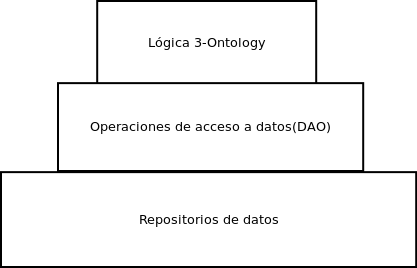
\includegraphics[scale=.6]{images/capadedatos.png}
	\caption{Capa de datos de RBOX 2.0 }
	\label{fig:capadatos}
\end{figure}

\begin{itemize}
\item \textbf{Repositorios de datos}: corresponde a un conjunto de repositorios que pueden contener información de utilidad para los SR.
\item \textbf{Operaciones de acceso a datos}: proveen un acceso a los datos almacenados dentro de múltiples repositorios. Dado que la capa es construida con el patrón DAO se provee abstracción al tipo de repositorio de datos usado.
\item \textbf{Lógica 3-Ontology}: provee un conjunto de operaciones que permiten obtener información relevante para las distintas fases de construcción de un SR.
\end{itemize}

\subsection{Alternativas de solución para distintos tipos de repositorios de datos}

Los repositorios donde están albergados los datos de relevancia de los SR pueden estar dispersos en distintas plataformas, por ejemplo: los datos referentes a las transacciones de los usuarios pueden estar albergadas en una base de datos de análisis (OLAP). Por otro lado, se puede realizar consultas de información referente a las preferencias de sus usuarios dentro de las redes sociales y almacenar en algún repositorio, también se pueden obtener datos geo-localizados de interacciones que los usuarios realicen en alguna aplicación móvil.

A continuación se presentan dos esquemas posibles de solución dependiendo de las necesidades de construcción de un SR.

En un primer esquema se asume que la información proviene de distintos repositorios que pueden ser bases de datos relacionales, objetuales, analíticas, archivos de texto, xml, etc. Cada uno de estos repositorios tiene información referente a los tres contenedores de la \textit{3-ontology} eventos, comunidades y lugares. En este caso, basta solo con implementar la capa \textbf{DAO} para los repositorios específicos.  En la Figura \ref{fig:multiplesrepositorios} se observa un diagrama explicitando la arquitectura propuesta. 

\begin{figure}[tp]
	\centering
	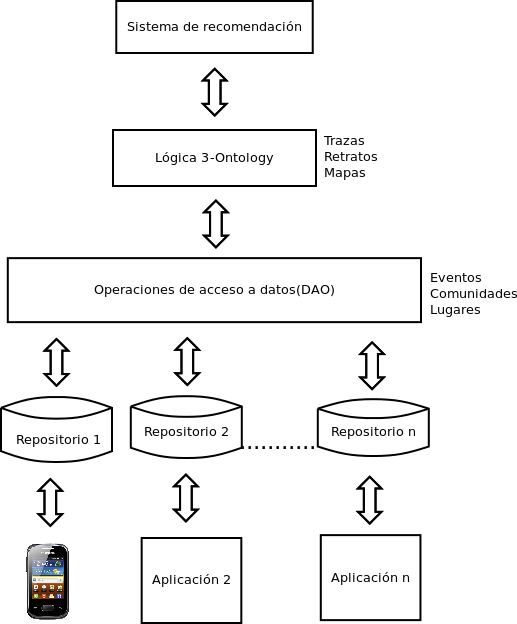
\includegraphics[scale=.6]{images/3-ontology-multiples-repos.png}
	\caption{Múltiples repositorios}
	\label{fig:multiplesrepositorios}
\end{figure}

En un segundo esquema se provee un modelo de datos relacional que es capaz de albergar la información de utilidad de un SR. En este caso se asume que se debe realizar una consolidación de los datos de los diversos repositorios para que sean mapeados dentro de la base de datos relacional de la \textit{3-ontology}. \cite{Molins:2012} provee una herramienta que permite realizar el mapeo desde bases de datos relacionales, archivos de texto y xml al esquema de datos de \textit{Synergy}. En el trabajo futuro expone las directrices para modificar su herramienta y aplicarla a un esquema destino distinto como es el de la \textit{3-ontology}. En la Figura  \ref{fig:unrepositorio} se muestra la arquitectura propuesta para el segundo caso propuesto.

\begin{figure}[tp]
	\centering
	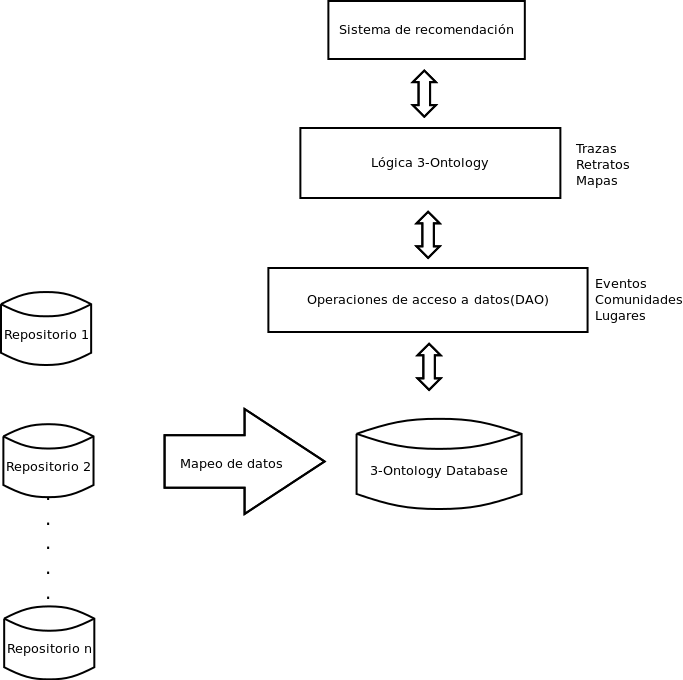
\includegraphics[scale=.6]{images/3-ontology-1-repo.png}
	\caption{Repositorio con la estructura de la \textit{3-Ontology}}
	\label{fig:unrepositorio}
\end{figure}


\subsection{Operaciones de acceso a datos}

Las operaciones de acceso a datos permiten realizar el típico conjunto de operaciones de base de datos \textbf{CRUD} \textit{(Create, Read, Update, Delete)} sobre los eventos, comunidades y lugares. Como ya se mencionó estos pueden estar en distintos repositorios (organizacionales, redes sociales, aplicaciones móviles, etc). Las operaciones de acceso a datos también  permiten obtener información referente a los usuarios e ítems.

El diseño de esta capa se realiza mediante el patrón DAO \textit{(Data Access Object)}\footnote{http://www.oracle.com/technetwork/java/dataaccessobject-138824.html} que permite la abstracción del repositorio de datos. Cada implementación de las interfaces DAO propuestas permitirá el acceso a un repositorio de datos específico. La solución incorpora una implementación genérica para el acceso a una base de datos relacional con el esquema \textit{3-Ontology} mediante JDBC (\textit{Java DataBase Connectivity}).

%El diseño de clases DAO se muestra en la figura x.x
%
%IMAGEN CON EL DISEÑO DE CLASES DAO

Cabe destacar que las operaciones más utilizadas serán de lectura. Sin embargo, las operaciones crear, actualizar y remover pueden ser usadas para un proceso de migrado o para almacenar la información obtenida del proceso de recomendación como por ejemplo nuevas comunidades.

\subsection{L\'ogica de la 3-Ontology}

Como se mencionó en el capítulo \ref{capitulo:modelo} la \textit{3-ontology} se compone de tres formas de representación (trazas, retratos y mapas) que dotan de lógica a los eventos, comunidades y lugares permitiendo obtener las siguientes ventajas:

\begin{itemize}
	\item Representar la composición y recursividad de las comunidades y lugares.
	\item Representar la secuencialidad temporal de los eventos.
	\item Situar a los eventos dentro de una comunidad y lugar.
	\item Representar distintos tipos de interacciones hacia los ítems.
	\item Representar la pertenencia de los ítems y usuarios a un lugar físico y/o virtual.
	\item Representar la pertenencia de usuarios a una o varias comunidades.
	\item Representar la pertenencia entre comunidades y lugares.
\end{itemize}

La representación más un conjunto de métodos permite dar una implementación a la \textit{3-Ontology}. El conjunto de los métodos y la representación son denominados lógica de la \textit{3-Ontology}.

Las trazas denotan la relación existente entre los eventos. Además, de los métodos sobre la causalidad temporal de los eventos se proveen métodos que permiten obtenerlos dadas las características propias de estos para el caso de los SR. Dado lo anterior, se expone un conjunto de métodos dentro de una interfaz que representan a una traza basado en el modelo propuesto. En el código \ref{cod:trace} se muestra la interfaz propuesta para una traza. Los eventos pueden ser obtenidos de forma ordenada mediante el uso de comparadores. Además, los métodos propuestos permiten realizar apoyo a operaciones de pre y post filtrado en CARS obteniendo sólo los eventos relevantes para el cálculo de la recomendación dado un contexto. 

\begin{lstlisting}[float, caption = Interfaz Trace, label = cod:trace]
public interface Trace{

    List<Event> getEvents();

    List<Event> getEvents(Comparator<Event> comparator);

    <E extends Event> List<E> getEvents(Comparator<Event> comparator, Class<E> type);

    <E extends Event> List<E> getEvents(Class<E> type);

    List<Event> getEventsForItem(long itemId);

    List<Event> getEventsForItemByTimestamp(long itemId, long timestamp1, long timestamp2);

    List<Event> getEventsByTimestamp(long timestamp1, long timestamp2);

    <E extends Event> List<E> getEventsForItem(long itemId, Class<E> type);

    <E extends Event> List<E> getEventsForItem(long itemId,Comparator<Event> comparator, Class<E> type);

    List<UserHistory<Event>> getEventsByUser();

    UserHistory<Event> getEventsForUser(long userId);

    UserHistory<Event> getEventsForUserByTimestamp(long userId, long timestamp1, long timestamp2);

    <E extends Event> UserHistory<E> getEventsForUser(long userId, Class<E> type);

    LongSet getUsersForItem(long item);

    <E extends Event>  LongSet getUsersForItem(long itemId, Class<E> type);  

    LongSet getItemsForUser(long userId);

    <E extends Event>  LongSet getItemsForUser(long userId, Class<E> type);
}
\end{lstlisting}

Los retratos representan las relaciones existentes entre las comunidades. Se proveen métodos que permiten obtener información referente a las relaciones entre usuarios y comunidades. Por ejemplo, se puede determinar a que comunidades pertenece el usuario $u$. En el código \ref{cod:portrait} se presenta la definición de la interfaz propuesta para un retrato.

\begin{lstlisting}[float,caption = Interfaz Portrait, label = cod:portrait]
public interface Portrait{
    
    Community getAllUsers();
    
    List<Community> getCommunities();

    <E extends Community> List<E> getCommunities(Class<E> type);

    List<Community> getCommunitiesForUser(long userId);

    <E extends Community> List<E> getCommunitiesForUser(long userId, Class<E> type);  
}
\end{lstlisting}

Los mapas representan las relaciones existentes entre los lugares. Se proveen métodos que permiten obtener información referente a a las relaciones entre los ítems y lugares. Por ejemplo, se pueden obtener todos los lugares a los que un ítem $c$ pertenece. En el código \ref{cod:map} se presenta la definición de la interfaz propuesta para un mapa.

\begin{lstlisting}[float, caption = Interfaz Mapa, label = cod:map]
public interface Map {  
  
    Place getAllItems();
    
    List<Place> getPlaces();
    
    <E extends Place> List<E> getPlaces(Class<E> type);
    
    List<Place> getPlacesForItem(long itemId);

    <E extends Place> List<E> getPlacesForItem(long itemId, Class<E> type);  
}
\end{lstlisting}

\section{Modelo entidad-relación para la 3-Ontology}

Para permitir una representación al nivel de repositorio de datos se provee un modelo entidad-relación que permite realizar un almacenamiento en una base de datos
relacional. En la Figura \ref{fig:modeloentidadrelacion} se muestran las entidades fundamentales (contenedores de sentido) mediante las tablas \textit{Event}, \textit{Community} y \textit{Place}. Los ítems y usuarios son reflejados por las tablas \textit{Item} y \textit{User}.

\begin{figure}[tp]
	\centering
	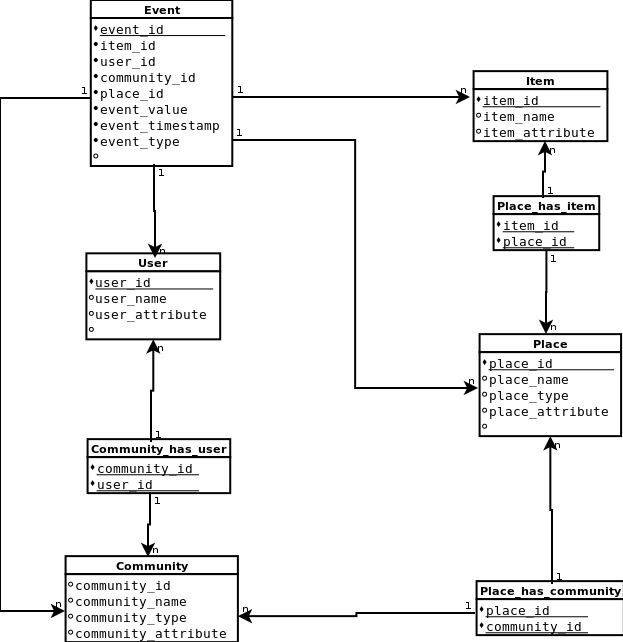
\includegraphics[scale=.6]{images/modeloentidadrelacion.png}
	\caption{Modelo entidad-relación }
	\label{fig:modeloentidadrelacion}
\end{figure}

La columna "\textit{event\_type}" de la tabla \textit{event}  permite modelar varios tipos de interacciones sobre el mismo ítem. En el modelo físico todas las relaciones n-arias del diagrama entidad-relación son reflejadas mediante las siguientes tablas:

\begin{itemize}
	\item \textit{Place\_has\_item}
	\item \textit{Place\_has\_community}
	\item \textit{Community\_has\_user}
\end{itemize}

Estas tablas permiten situar los eventos, usuarios e items en un contexto temporal, espacial y social. El modelo presenta pocos atributos obligatorios para no restringir la representación de los repositorios de datos que no poseen todos los datos necesarios del modelo propuesto. De esta manera, se puede instanciar este modelo de datos para un dominio específico y agregar los atributos que se consideren relevantes. Los únicos atributos obligatorios del evento son el identificador del usuario, objeto, valor y el tipo del evento. Por lo tanto, en las otras tablas solo los identificadores son obligatorios dotando de flexibilidad de representación al modelo propuesto.

\section{Construcción de un SR}
\label{sec:consSR}

Para construir SR en RBOX 2.0 se define la interfaz \textit{RBOXRecommender} (véase el código \ref{cod:recommender}) que permite prestar servicios de recomendación. Los métodos definidos reciben distintos parámetros de entrada para realizar el cálculo de la recomendación para el usuario activo. La salida es una lista de \textit{ScoredItem} que corresponden a ítems con un puntaje calculado por un algún algoritmo de recomendación. Se recomiendan los ítems que tienen el puntaje mayor.

\begin{lstlisting}[float, caption = Interfaz RBOXRecommender, label = cod:recommender]
public interface RboxRecommender {
	
    String getName();
    
    List<ScoredItem> recommend(long idUser, int n);
    
    List<ScoredItem> recommend(long idItem); 
    
    List<ScoredItem> recommend(long idUser, int n,  List<Item> candidates,
    		List<Item> exclude);
    
    List<ScoredItem> recommend(long idUser, List<Item> candidates);
}
\end{lstlisting}

El método definido para construir un SR basado en el modelo propuesto se presenta en la Figura \ref{fig:procesoconstruccionSR}. Primero se deben seleccionar los repositorios de datos que disponen de datos relevantes. Una vez identificados se debe modelar los contenedores de sentido del modelo, en otras palabras se determina que como serán los eventos, comunidades y lugares. Luego se debe determinar si se consolidarán los datos usando la base de datos relacional o implementar la capa \textbf{DAO} para cada repositorio. Una vez que se dispone de los datos, se debe seleccionar un algoritmo de recomendación o de aprendizaje de máquina desde algún API como \textit{Lenskit}, \textit{Weka}, \textit{Apache Mahout} o \textit{Mallet}. Si el algoritmo no cumple con las expectativas se puede modificar y/o cambiar por otro. Finalmente, se implementa la interfaz \textit{RBOXRecommender} utilizando las trazas, retratos y mapas como entrada de datos. Es importante señalar que durante el desarrollo del algoritmo de recomendación se procesan las distintas características provistas por el modelo propuesto.

\begin{figure}[tp]
	\centering
	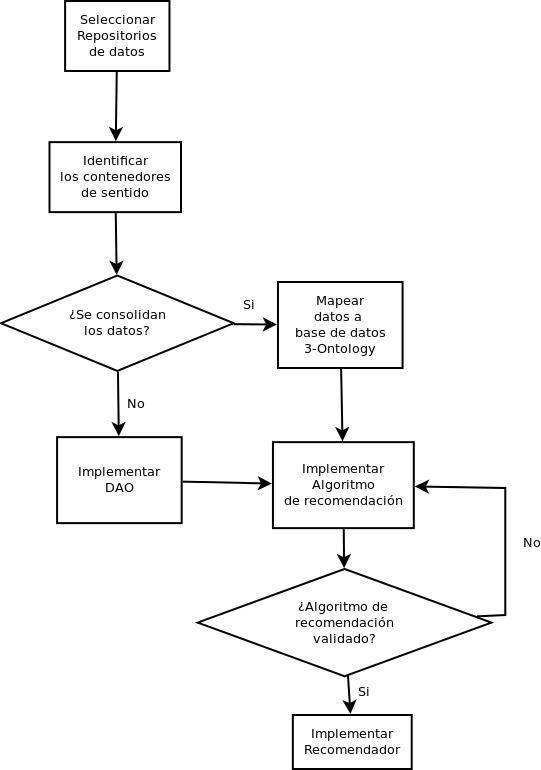
\includegraphics[scale=.6]{images/procesoconstruccionSR.png}
	\caption{Flujograma de creación de un SR }
	\label{fig:procesoconstruccionSR}
\end{figure}

\section{Habilidades necesarias desarrollar con RBOX 2.0}

En esta sección se definen el conjunto de habilidades y conocimientos que debe tener un desarrollador para implementar SR con RBOX 2.0.

\begin{itemize}
\item{\textbf{Lenguaje de programación}}: el desarrollador debe poseer un nivel intermedio del lenguaje de programación \textit{Java}. Esto quiere decir que debe tener conocimiento en:
\begin{itemize}
\item Fundamentos de programación.
\item Uso de interfaces y clases abstractas.
\item Colecciones.
\item Anotaciones.
\item Tipos genéricos.
\item Utilización de librerías.
\end{itemize}

\item{\textbf{Diseño orientado a objetos y patrones de diseño}}: el desarrollador debe tener conocimientos intermedios de orientación a objetos (abstracción, polimorfismo, encapsulación y herencia) que le permita extender el sistema. Además, debe tener conocer los patrones de diseño usados del sistema.

\item{\textbf{Control del ciclo de vida del software}}: este conocimiento se refiere al uso de herramientas que apoyen al proceso de compilación, pruebas y despliegue del software. En el caso de RBOX 2.0 se utiliza \textit{Gradle}, este conocimiento es opcional debido a que se pueden construir SR sin el uso de este tipo de herramientas. 

\item{\textbf{Minería de datos y aprendizaje automático}}: Se asume que el desarrollador tiene conocimientos de técnicas de minería de datos y aprendizaje automático que le permiten construir algoritmos de recomendación. Por ejemplo como se específico en la sección 2.1, los SR basados en \textit{rating} se basan en un problema de predicción, luego el desarrollar debe conocer las técnicas del aprendizaje de máquina disponibles para abordar el problema de predicción.

\end{itemize}

\section{Integración con otras aplicaciones}

La solución provista permite la construcción de SR en \textit{Java} que pueden ser utilizados por aplicaciones Web o móviles que soporten el uso de servicios del tipo \textit{RESTful}. Para lo anterior, se debe encapsular el SR usando \textit{JavaEE 6}\footnote{Java Enterprise Edition 6}, permitiendo así disponer del SR en un contenedor.

Los pasos sugeridos para la construcción son los siguientes:

\begin{enumerate}
\item Construir un SR con el modelo propuesto en este trabajo.
\item Construir un \textit{SessionBean} (\textit{Enterprise Java Bean}) de tipo \textit{Stateless} que encapsule en métodos de negocio la interfaz de recomendación propuesta por RBOX 2.0.
\item Construir servicios de tipo \textit{RESTful} a partir del \textit{SessionBean} creado.
\item Desplegar los servicios en un contenedor dentro de un servidor de aplicaciones.
\item Consumir los servicios desde aplicaciones clientes.
\end{enumerate} 

Esta integración requiere que el desarrollador conozca de arquitectura de aplicaciones empresariales en específico JavaEE, luego implementar la integración sugerida no puede ser aplicada por un desarrollador que no tenga experiencia.


\section{Comparación con otras herramientas}

En esta sección se realiza una comparación de RBOX 2.0 con otras herramientas de software que permiten la construcción de SR. 

RBOX 2.0 para soportar las nuevas características de los SR modernos se rige bajo los siguientes principios de diseño:
\begin{itemize}
	\item \textbf{Mantenibilidad}: se refiere al esfuerzo ahorrado para revisar y corregir errores.
	\item \textbf{Flexibilidad}: se refiere al esfuerzo ahorrado para extender y realizar cambios de configuración del sistema.
	\item \textbf{Reusabilidad}: se refiere al esfuerzo ahorrado de reutilizar módulos y/o componentes de software.
	\item \textbf{Escalabilidad}: se refiere a la capacidad del sistema de soportar una calidad de servicio cuando la carga de eventos aumenta.
\end{itemize}

\cite{Ekstrand:2011} presentan \textit{Lenskit}\footnote{http://lenskit.grouplens.org/} un \textit{toolkit} para construir, investigar y estudiar SR de filtrado colaborativo basados exclusivamente en eventos de tipo \textit{rating}. Se enfoca principalmente en resolver las dificultades referentes a la investigación con SR. \textit{Lenskit} se basa en tres objetivos de diseño:

\begin{itemize}
	\item \textbf{Modularidad}: los algoritmos de recomendación se descomponen dentro de varias piezas constituyentes como normalización, funciones de similaridad y reglas de predicción. Varios de los componentes anteriores no son parte de un algoritmo particular. Esta diseñado para ser altamente modular y reconfigurable.
	\item \textbf{Claridad}: se debe mantener un núcleo simple pero con interfaces que provean integración y extensión en sistemas en tiempo real.
	\item \textbf{Eficiencia}:  se prefiere el código claro antes que obscuras optimizaciones. Puede procesar \textit{Movielens 10m} con 10 millones de eventos de tipo \textit{rating}.
\end{itemize}

Las ventajas de \textit{Lenskit} son su modularidad, configurabilidad y  alto rendimiento para trabajar con SR de filtrado colaborativo. La principal desventaja es no proporcionar una forma estándar de representar los datos que permita modelar características contextuales de las interacciones. Cabe señalar que los algoritmos de filtrado colaborativo utilizados en RBOX 2.0 son extraídos de \textit{Lenskit} ya que son escalables y modulares. La mantenibilidad es asegurada mediante el uso de patrones de diseño y orientación a objetos, la flexibilidad mediante el uso de interfaces simples, la reusabilidad mediante el uso de componentes con alta cohesión y bajo acoplamiento, la escalibilidad mediante el uso de estructuras de datos especializadas como \textit{Sparse Vector}. 

\cite{Babar:2010} presentan \textit{Synergy} una herramienta para la creación, ejecución y comparación de diferentes algoritmos de filtrado colaborativo. La idea fundamental de \textit{Synergy} es que los algoritmos de recomendación deben ser reconfigurados o cambiados por otros durante el tiempo.  Las ventajas de \textit{Synergy} son la posibilidad de modelar diversas formas de interacción, la hibridación de algoritmos de filtrado colaborativo y la generación de SR en formato \textit{plug-in}. Su principal dificultad es que no se encuentra disponible el código por lo tanto no se dispone de información referente a las cuatro propiedades sistémicas evaluadas.

% % Referenciar a Salvador

\cite{Cullache:2011} y \cite{Cortes:2013} presentan RBOX 1.0 una herramienta de software para experimentar con SR de filtrado colaborativo inspirado por \textit{Synergy} y \textit{Weka}. El uso excesivo del patrón de diseño ``\textit{Abstract Factory}'' dificulta la mantenibilidad y flexibilidad del código ya que la mayoría de los objetos de la aplicación son creados con este patrón. Respecto a la reusabilidad se logra mediante la agregación de \textit{plug-ins}. La escalabilidad no es resguardada teniendo serios problemas de rendimiento ya que no posee estructuras de datos especializadas como ``\textit{Sparse Vector}''.

 RBOX 2.0 cumple con la mantenibilidad mediante el uso de patrones de diseño y orientación a objetos. La flexibilidad se asegura mediante el uso de interfaces simples que puedan ser extendidas como es el caso de los eventos \textit{ratings} y \textit{taggings}.  La reusabilidad se asegura mediante el diseño de componentes que posean una alta cohesión y bajo acoplamiento. Finalmente, la escalabilidad se asegura mediante el uso de \textit{Lenskit} para algoritmos de SR de filtrado colaborativo y de \textit{Fast-utils}\footnote{http://fastutil.di.unimi.it/} para estructuras de datos complejas. En la tabla \ref{tabla:comparacionotrasherramientas} se muestra un resumen del cumplimiento de las propiedades sistémicas para cada herramienta. Además, los siguientes patrones de diseño, técnicas de programación y librerías apoyan al cumplimiento de los principios de diseño de RBOX 2.0:
 
 \begin{itemize}
 	\item \textbf{Tipos genéricos}: provee la capacidad de re-usar el mismo código para distintas entradas.
 	\item \textbf{Builders}: patrón creacional que permite la construcción de objetos complejos que no siempre disponen de todos los atributos. Es una alternativa del anti-patrón \textit{telescopic constructor}.
 	\item \textbf{Data access object}: patrón estructural que permite la abstracción de los datos.
 	\item \textbf{Dependency Injection}: patrón creacional que permite resolver las dependencias de objetos en tiempo de ejecución y/o compilación.
 	\item \textbf{Fast-utils}\footnote{http://fastutil.di.unimi.it/}:  es un \textit{framework} que extiende de \textit{Java Collections}\footnote{http://docs.oracle.com/javase/tutorial/collections/} y provee mapas, conjuntos, listas y colas con baja utilización de memoria, rápido acceso e inserción.
 	\item \textbf{Preferencia de objetos inmutables}\footnote{http://docs.oracle.com/javase/tutorial/essential/concurrency/immutable.html}: su uso asegura que el estado de un objeto no cambiará después que es construido. Son útiles en el desarrollo de aplicaciones concurrentes.
 \end{itemize}
 
 
\begin{table}[H]
\caption{Comparación con otras herramientas de software}
\label{tabla:comparacionotrasherramientas}
\begin{center}
	\begin{tabular}{|>{\centering\arraybackslash}p{3cm}  | >{\centering\arraybackslash}p{2cm}  |>{\centering\arraybackslash}p{2cm} |>{\centering\arraybackslash}p{2cm} |>{\centering\arraybackslash}p{2cm} |}
	\hline	& \multicolumn{4}{c|}{Herramientas de software} \\	
	
	\hline Propiedad	 				 				& Lenskit  & 
	Synergy & RBOX 1.0 & RBOX 2.0 \\ 
	\hline Mantenibilidad 		 				& X &   &   & X  \\ 
	\hline Flexibilidad 						& X &   &   & X \\ 
	\hline Reusabilidad 						& X &   & X & X \\ 
	\hline Escalabilidad						& X &   &   & X \\ 
	\hline 
	\end{tabular} 
\end{center}
\end{table}

En la tabla \ref{tabla:comparacionotrasherramientas} se puede observar que \textit{Lenskit} al igual que RBOX 2.0 cumplen con las todas propiedades sistémicas evaluadas. Por otro lado, al no tener disponible el código fuente de \textit{Synergy} no se puede determinar si cumple o no con las propiedades evaluadas. En el caso de RBOX 1.0 se intenta utilizar ciertos patrones de diseño para asegurar algunas propiedades, sin embargo el uso inadecuado de patrones de diseño termina limitando la herramienta. Se observa que las propiedades sistemáticas del software RBOX 2.0 y \textit{Lenskit} son idénticas, sin embargo la principal ventaja que posee RBOX 2.0 sobre \textit{Lenskit} está relacionada con la conceptualización proporcionada por el modelo propuesto, que basa su implementación en la \textit{3-Ontology}. Lo anterior logra que RBOX 2.0 sea una herramienta más comprensible que \textit{Lenskit} permitiendo crear rápidamente prototipos para ámbitos empresariales y científicos agregando todas las ventajas presentadas en la sección 3.3. 


%\section{Resumen}
%
%En este capítulo se presentó RBOX 2.0 una herramienta de software basada en el modelo de representación propuesto. Se presentó la arquitectura del software mediante un diagrama de componentes y de módulos del sistema, posteriormente se presentó el diseño de las clases principales que dan sentido al \textit{framework} propuesto. Finalmente, se presentaron herramientas similares y se evaluaron bajo 4 propiedades sistemáticas mantenibilidad, reusabilidad, flexibilidad y escalabilidad. RBOX 2.0 cumple con las cuatro propiedades que le permite ser un software de calidad para la construcción de SR basados en una representación de datos genérico aplicable a diversos dominios de aplicación.


% % Diseño de clases contenedores de sentido y darse-cuenta

% % Módulos de RBOX 2.0

% % Diseño de un modelo entidad-relación para BD

% % Comparación con herramientas similares

%\chapter{Ejemplos de aplicación}

En el presente capítulo se muestran dos ejemplos de aplicación del \textit{framework} donde se realiza la construcción de SR que permiten validar la eficacia del modelo propuesto.

\section{Sistemas de recomendación para \textit{Movielens}}

\textit{Movielens}\footnote{http://movielens.umn.edu/} es un servicio libre, no comercial y personalizado ofrecido por \textit{Grouplens}\footnote{http://grouplens.org/} de la Universidad de \textit{Minnesota}\footnote{www.umn.edu/}. Este permite realizar recomendaciones de películas basándose en interacciones de tipo \textit{rating}. El \textit{dataset} usado de \textit{Movielens} en este trabajo fue presentado en el \textit{workshop} \textit{HetRec} 2011\footnote{The 2nd International Workshop on Information Heterogeneity and Fusion in Recommender Systems}. Este se basa en dos tipos de interacciones \textit{rating} y \textit{tagging}, el detalle estadístico del \textit{dataset} es el siguiente:

\begin{itemize}
	\item 2113 usuarios.
	\item 10197 películas.
	\item 13222 \textit{tags}.
	\item 47957 asignaciones de \textit{tags}, por ejemplo tuplas [\textit{user}, \textit{tag}, \textit{movie}].
	\item Un promedio de 22.696 asignaciones de \textit{tags} por usuario.
	\item Un promedio de 8.117 asignaciones de \textit{tags} por ítem.
	\item 855598 \textit{ratings}.
	\item Un promedio de 404.921 \textit{ratings} por usuario.
	\item Un promedio de 84.637 \textit{ratings} por película.
\end{itemize}

Según la método propuesto para la construcción(véase sección \ref{fig:procesoconstruccionSR}) el primer paso consiste en realizar la selección del repositorio de datos a usar. En este caso corresponde a un conjunto de archivos de texto que poseen la información sobre los usuarios, películas e interacciones.

Una vez seleccionado el repositorio de datos se debe decidir que estrategia de acceso a los datos se usará, una consolidación dentro una BD \textit{3-Ontology} o un acceso mediante una implementación DAO. En este caso, se decide realizar una implementación de la capa DAO dado que el objetivo fundamental es experimentar para realizar mejoras en el filtrado colaborativo basado en \textit{rating}. Por lo tanto, se hace uso de un FileDAO que implementa las interfaces EventDAO, CommunityDAO y PlaceDAO para un acceso de datos a archivos de texto plano. En el código \ref{cod:constructorFileDao} se presenta el constructor del FileDAO. Cabe destacar que en esta etapa se determinan los tres contenedores de sentido provenientes desde los archivos de texto.

\begin{lstlisting}[float, caption = Constructor FileDAO, label = cod:constructorFileDao]
	public FileDAO(String pathRatingFile, String pathTaggingFile, char delim) throws IOException{
		ratingFile = new ReaderRatingFile(pathRatingFile, delim);
		taggingFile = new ReaderTaggingFile(pathTaggingFile, delim);
		events = Lists.newArrayList(ratingFile);
		events.addAll(Lists.newArrayList(taggingFile));
		ratingFile.close();
		taggingFile.close();
		userIds = new LongOpenHashSet();
		itemIds = new LongOpenHashSet();
		communities = Lists.newArrayList();
		places = Lists.newArrayList();
		loadData();
	}
\end{lstlisting}

Una vez implementado el acceso a los datos con su respectiva representación en los contenedores de sentido se debe implementar un algoritmo de recomendación. Existen diversas API que proveen implementaciones de algoritmos de recomendación, en este caso se hará uso de las implementaciones provistas por \textit{Lenskit} para filtrado colaborativo. Específicamente se usará el enfoque de vecinos más cercanos \textit{user-user}, que es una heurística que dada las preferencias de usuarios cercanos realiza una aproximación de la preferencia del usuario activo (véase la sección 2.2).

A partir del FileDAO se construye una traza, un retrato y un mapa que son la representación lógica de los tres contenedores de sentido de la \textit{3-Ontology}. Luego cada objeto relacionado con el algoritmo de recomendación hace uso de la traza, retrato y mapa, para obtener los eventos, comunidades, lugares, usuarios e ítems relevantes para realizar el cálculo de la recomendación. Finalmente, se implementa la interfaz RboxRecommender para realizar el cálculo de la recomendación para un usuario activo. En el código \ref{cod:srknn} se muestra un ejemplo de implementación de un SR basado en el método propuesto.

\begin{lstlisting}[float, caption = SR \textit{knn-user/user}, label = cod:srknn]
		/*Creacion del FileDAO para acceder a los datos*/
		FileDAO fileDAO = new FileDAO("/home/rodrigo/user_ratedmovies-timestamps.dat", 
				"/home/rodrigo/user_taggedmovies-timestamps.dat", '\t');
		/*Creacion de las 3 representaciones de la 3-ontology a partir de los contenedores de sentido*/
		Trace trace = new GenericTrace(fileDAO.getEvents());
		Portrait portrait = new GenericPortrait(fileDAO.getCommunities());
		Map map = new GenericMap(fileDAO.getPlaces());
		
		/*Creacion de los objetos relacionados con el algoritmo de recomendacion*/
		VectorSimilarity similarity =  new PearsonCorrelation();
		UserSimilarity userSimilarity = new UserVectorSimilarity(similarity);
		VectorNormalizer norm = new MeanVarianceNormalizer();
		UserVectorNormalizer vectorNormalizer = new DefaultUserVectorNormalizer(norm);
		NeighborhoodFinder finder = new SimpleNeighborhoodFinder(trace,10, userSimilarity, vectorNormalizer);
		ItemScorer userUserItemScorer = new UserUserItemScorer(trace, finder, vectorNormalizer);
		TopNItemRecommender itemRecommender = new TopNItemRecommender(trace, portrait, map, userUserItemScorer);
		ItemScorer baseline = new ItemMeanRatingItemScorer.Builder(trace, 0).get();
		PreferenceDomain domain = new PreferenceDomain(0, 5);
		SimpleRatingPredictor ratingPredictor = new SimpleRatingPredictor(userUserItemScorer, baseline, domain);
		
		/*Construccion de un SR basado en la logica de la 3-Ontology*/
		RboxRecommender rboxRecommender = new RboxRecommenderBasedItemScorer(trace, map, portrait, itemRecommender, ratingPredictor.getBaselineScorer());
\end{lstlisting}

El uso del SR se realiza mediante una lista de ScoredItem que corresponden a ítems con un puntaje asignado por los algoritmos de recomendación. Un ejemplo de uso del algoritmo se presenta en el código \ref{cod:ejemplouso} donde se imprimen las 10 primeras recomendaciones para el usuario 75. Este algoritmo está basado en memoria por esta razón se debe re-calcular la lista de recomendaciones cada vez que el sistema es consultado.

\begin{lstlisting}[float, caption = Ejemplo de uso, label = cod:ejemplouso]
for(ScoredItem scoredItem: rboxRecommender.recommend(75, 10)){
			System.out.println(scoredItem.toString());
		}
\end{lstlisting}

Es importante notar que la lógica de la \textit{3-Ontology} provee métodos de pre-filtrado que permiten la implementación de CARS \citep{Adomavicius:2011}, obteniendo así eventos relevantes para el cálculo de la recomendación en un contexto dado. Por ejemplo, para realizar una recomendación de películas un día sábado, se pueden obtener solo los eventos sucedidos los sábados. De esta forma se calcula una lista de recomendación para el usuario basada en el contexto temporal donde él asigna una valoración a la película.


\section{Sistemas de recomendación para un proceso de generación de noticias}

\cite{Alonso:2012} en su trabajo de titulación modela un proceso de negocio de generación de noticias de la empresa \textit{Observatorio News} que incluye un etiquetado de los periodistas para agregar valor al negocio. \cite{Rivera:2012} presenta un modelo 4+1 vistas para describir la arquitectura de software que debe ser soportado para el proceso de negocio. \cite{Mendez:2013} realiza la descripción arquitectural para el sistema, especificando cada componente del proceso. RBOX 2.0 según estos trabajos es la herramienta que permite generar SR de tipo \textit{plug-in} que pueden ser integrados en la arquitectura propuesta. Bajo estas premisas se propone como caso de estudio el desarrollo de un SR basado en \textit{tags} para el proceso de negocio de la empresa \textit{Observatorio News}, cabe destacar que el desarrollo de este SR está suscrito al proyecto FONDEF D09I1185, luego los datos usados pertenecen a la empresa socia del proyecto \textit{Observatorio News}.

\textit{Observatorio News} necesita que los periodistas novatos aprendan de los \textit{Senior} a etiquetar noticias, esto se justifica debido a que dependiendo del nivel de etiquetado que apliquen los periodistas se le puede recomendar noticias de mejor calidad a los usuarios. Para lograr este objetivo la lógica de la \textit{3-Ontology} provee el método \textit{getEventsForUser(userId)} que permite obtener solo los eventos que han efectuado los periodistas Senior. De esta forma el algoritmo puede aprender sobre como etiquetan los periodistas Senior y recomendar a los novatos etiquetas que apoyen su proceso de etiquetado.

El \textit{dataset} de \textit{Observatorio News} corresponde a noticias etiquetadas por periodistas en sectores e incluye la siguiente información:

\begin{itemize}
	\item id\_noticia: corresponde al identificador de la noticia.
	\item id\_idioma: idioma de la noticia, pudiendo ser ingles, español o portugués.
	\item fec\_publicacion: fecha de publicación del artículo. Formato DD-MM-YY.
	\item id\_paises: códigos de países separados por coma.
	\item paises: nombres de países separados por coma.
	\item id\_sector: código del sector asociado al artículo.
	\item sector: nombre del sector asociado al artículo.
	\item id\_sub\_sectores: códigos de subsectores asociados al artículo.
	\item sub\_sectores: nombres de subsectores asociadas al artículo.
	\item titulo: título del artículo.
	\item cuerpo: contenido del cuerpo del artículo (párrafos separados por el carácter '|').
	\item id\_usuario: usuario que creó la noticia y selecciono los \textit{tags}.
\end{itemize}

Los datos obtenidos se consolidan en el esquema relacional de la \textit{3-Ontology}, para esto se siguió el siguiente procedimiento:

\begin{itemize}
	\item Se eliminan los campos irrelevantes.
	\item Se cambia el enfoque desde la noticia hacia el evento.
	\item Cambiar el formato de la fecha a \textit{UNIX timestamp}.
	\item Se crean los archivos necesarios para la carga en un motor de base de datos relacional con esquema \textit{3-Ontology}.
\end{itemize}

Los archivos que resultan del proceso de normalización de datos son \textit{event\_bna.dat}, \textit{user\_bna.dat} y \textit{item\_bna.dat}.

Descripción del archivo event\_bna.dat:
\begin{enumerate}
	\item id\_event: identificador del evento.
	\item id\_noticia: identificador de la noticia.
	\item id\_usuario: identificador del usuario.
	\item id\_subsector: identificador del subsector.
	\item timestamp\_noticia: timestamp del evento en formato UNIX timestamp.
	\item type\_event: corresponde al tipo de evento (en este caso \textit{tagging}).
\end{enumerate}

Los eventos son uni-valuados, luego si se seleccionan más de un subsector se identifican como eventos distintos.

Descripción del archivo user\_bna.dat:
\begin{enumerate}
	\item id\_usuario: identificador del usuario.
	\item nombre\_usuario: nombre del usuario.
\end{enumerate}

Descripción del archivo item\_bna.dat:
\begin{enumerate}
	\item id\_noticia: identificador de la noticia.
	\item titulo\_noticia: título de la noticia.
\end{enumerate}

En resumen el \textit{dataset} dispone de 438571 eventos, 150 periodistas, 209846 noticias. Con los archivos se puede realizar la carga de datos en una base de datos que disponga del esquema de datos de la \textit{3-Ontology} (véase sección 4.4). En este caso la columna \textit{value} dentro de la tabla \textit{event} corresponderá al subsector colocado por el periodista al momento de escribir la noticia. 

En este caso, se hará uso del paquete \textit{sql} de RBOX 2.0 que provee un conjunto de clases que permiten el acceso a una base de datos relacional con el esquema \textit{3-Ontology} mediante JDBC. El motor de bases de datos usado fue \textit{Mysql}\footnote{http://www.mysql.com/}. En el código \ref{cod:JDBCDAO} se muestra como se realiza el acceso a los datos de \textit{ABC News} mediante los componentes de RBOX 2.0.

\begin{lstlisting}[float, caption = Ejemplo de uso mediante JDBCDAO, label = cod:JDBCDAO]
	MysqlDataSource dataSource = new MysqlDataSource();
	Properties properties = new Properties();
	properties.load(new FileInputStream("algorithm.properties"));
	dataSource.setServerName(tabla.getString("db.principal.ip"));
	dataSource.setDatabaseName(tabla.getString("db.principal.schema"));
	dataSource.setUser(tabla.getString("db.principal.user"));
	dataSource.setPassword(tabla.getString("db.principal.pass"));
	Connection con = dataSource.getConnection();
	JDBCDAO dao = new JDBCDAO(con, 
								new BasicSQLStatementFactory(), 
								new BasicSQLStatementFactory(),
								new BasicSQLStatementFactory(),
								new BasicSQLStatementFactory(),
								new BasicSQLStatementFactory(),
								true);
	Trace trace = new GenericTrace(dao.getEvents());
	Portrait portrait  = new GenericPortrait(dao.getCommunities());
	Map map = new GenericMap(dao.getPlaces());
\end{lstlisting}


 

\subsection{Algoritmo de Tag Clustering}

\cite{Hernandez:2014} realiza un conjunto de implementaciones de algoritmos de recomendación de \textit{tags} para una red social de generación de noticias basados en el modelo de construcción propuesto en este trabajo de tesis. El algoritmo que se presenta como caso de estudio   se basa en un modificación del algoritmo presentado por \cite{Begelman:2006}. La modificación corresponde al reemplazo del algoritmo de \textit{clustering} por RRW \textit{(Repeated random walks)} \citep{Macropol:2009}. Este algoritmo a partir de un \textit{tag} busca los \textit{tags} relacionados y los retorna como recomendaciones. Luego se genera un modelo que puede ser consultado para obtener recomendaciones. Este  debe ser actualizado cuando deteriore sus resultados y/o existan nuevos eventos en el sistema.

%\section{Resumen}
%
%En este capítulo se presentó dos casos de estudio que permiten validar la eficacia del modelo propuesto. El primero corresponde a un SR basado en un algoritmo de filtrado colaborativo con eventos de tipo \textit{ratings} y el segundo basado en un algoritmo de \textit{tag clustering} con eventos de tipo \textit{tagging}. Se especificó la representación de datos usando las posibles alternativas de solución presentadas en el capítulo 4, se describió los \textit{datasets} a utilizar, luego se describieron los algoritmos utilizados, para finalmente describir como implementar la interfaz de recomendación.








\chapter{Conclusiones}
\label{cap:conclu}
En este capítulo se muestran las conclusiones del trabajo de tesis realizado. De esta forma, se explicitan los aportes realizados al área de los SR, se describe el cumplimiento de los objetivos específicos de este trabajo dando evidencia de su cumplimiento. Luego se presentan los posibles trabajos futuros a los que da lugar este trabajo de tesis. Finalmente, se exponen las reflexiones finales referentes al trabajo realizado.

\section{Aportes al \'area de los Sistemas de Recomendaci\'on}

El desarrollo de los SR como área de investigación ha sido acelerada en la última década debido al creciente desarrollo de la Web. En este trabajo se ha presentado un modelo de datos y un método de construcción de SR que otorga un marco de referencia para implementar SR. Dado esto, el primer aporte de este trabajo al área de los SR se basa en un modelo que permite una representación situada de los eventos que permite aprovechar las características contextuales de estos, este modelo tiene como base conceptual la \textit{3-Ontology} un \textit{framework} proveniente del área de los sistemas colaborativos. Luego se observa que los SR permiten capturar la inteligencia colectiva sobre un dominio de aplicación específico en base a tres contenedores de sentido comunidades, eventos y lugares. Estos además permiten persistir la inteligencia colectiva para ser usada posteriormente para entregar recomendaciones de utilidad a un usuario.

Un aporte de este trabajo de tesis corresponde a una herramienta de software llamada RBOX 2.0 que permite la construcción de SR basado en el modelo propuesto. RBOX 2.0 es de código abierto y extensible, permitiendo el desarrollo de SR tanto para el ámbito empresarial como científico. 

\section{Acerca de los objetivos espec\'ificos}

A continuación se describe el nivel de logro alcanzado en el desarrollo de este trabajo de tesis.
\begin{enumerate}
	\item \textit{Sistematizar el proceso de construcción de SR desde la literatura actual del área.}
	
	En la sección \ref{sec:consSR} se realizó una sistematización que permite la construcción de SR bajo el modelo propuesto. Este se basa en la evolución de los SR y sus representaciones presentadas en el marco teórico de este trabajo.
	
	\item \textit{Caracterizar las dimensiones emergentes para los SR.}
	
	En el capítulo 2 se presenta el marco teórico donde se definen las principales dimensiones emergentes de los SR. En el trabajo relacionado de la sección 4.1 se muestra como se han agregado nuevas dimensiones a los SR a las representaciones propuestas. 
	
	\item \textit{Diseñar un modelo orientado a eventos de representación de datos para SR.}
	
	En el capítulo 3 se presenta un modelo orientado a eventos que se basa en el \textit{framework 3-Ontology}. Este modelo permite situar los eventos dentro de un contexto social, espacial y temporal. En otras palabras este modelo es capaz de situar la colaboración existente dentro de aplicaciones pertenecientes a la Web 2.0.
	
	\item \textit{Diseñar un conjunto de operaciones para la obtención de datos desde el modelo de datos propuesto.}
	
	En el capítulo 3 se presenta la definición formal de un conjunto de operaciones que permiten obtener eventos, comunidades y lugares relevantes dependiendo del algoritmo de recomendación usado. Es importante notar que estas operaciones son parte del nivel meta de la \textit{3-Ontology} correspondientes a las trazas, mapas y retratos que dan sentido al nivel base (eventos, comunidades y lugares).
	
	\item \textit{Diseño e implementación de una herramienta para construir SR.}
	
	En el capítulo 4 se presenta el diseño e implementación de RBOX 2.0 una herramienta de software que permite el diseño e implementación de SR basados en el modelo de representación propuesto. RBOX 2.0 está construido bajo patrones de diseño que aseguran un conjunto de calidades sistemáticas requeridas. 
	
	\item \textit{Construir SR’s basados en el \textit{framework} propuesto.}
	
	En el capítulo 5 se presentan dos casos de estudio donde se presenta la construcción de dos SR basado en el modelo propuesto. El primer SR se basa en un algoritmo de vecinos más cercanos mediante el uso de eventos de tipo \textit{rating}, en este caso se recomiendan las películas con el \textit{rating} más alto predicho por el algoritmo. El segundo SR se basa en un algoritmo de \textit{clustering} basado en eventos de tipo \textit{tagging}, en este caso se recomiendan los \textit{tags} que se encuentren en el mismo \textit{cluster} que el \textit{tag} buscado. Dada la construcción de estos dos SR se valida la eficacia del modelo propuesto para la representación y construcción de SR basado en distintos tipos de eventos.
	
	\item \textit{Publicar los resultados de la investigación en una revista de la especialidad.}
	
	Se encuentra en desarrollo 2 publicaciones. La primera se basa en el modelo de representación de datos propuesto. La segunda es el diseño e implementación de RBOX 2.0 como herramienta para la representación y construcción de SR.
	
	
\end{enumerate}

\section{Trabajo futuro}

En este trabajo se propone e implementa un modelo de representación y construcción de SR basado en el \textit{framework} conceptual \textit{3-Ontology}. En este trabajo se exploró la eficacia del \textit{framework} para construir SR sin utilizar todas sus dimensiones, dado esto se vislumbran los siguientes trabajos futuros de índole científico e ingenieril:

\begin{itemize}
\item Investigar la dimensión de la comunidad y como esta permite retro-alimentar el proceso de recomendación. Por ejemplo,detectar comunidades emergentes dadas las valoraciones de los usuarios y almacenarlas dentro del modelo, para luego ser usadas como información adicional para futuras recomendaciones. Este trabajo se encuentra bajo desarrollo como tesis de Magíster en Ingeniería Informática \citep{Ochoa:2013}.

\item Investigar la dimensión referente a los lugares mediante la propuesta de un \textit{framework} que explicite los tipos de información espacial que son usados en SR. Construir un conjunto de algoritmos basados en lugares y explicitar las mejoras obtenidas en los SR.

\item Realizar una expansión del \textit{framework} propuesto para la evaluación de SR de forma \textit{offline} y \textit{online}, esto otorgaría una forma unificada para comparar diversos SR.

\item Investigar la construcción de SR híbridos utilizando las tres dimensiones del \textit{framework} para validar la eficacia y eficiencia de construir SR de recomendación con el modelo propuesto.

\item Estudiar la capacidad  de la \textit{3-Ontology} para representar la Web 2.0. Esto se justifica en la capacidad de representación de entornos colaborativos que posee la \textit{3-Ontology}. En este trabajo solo estudio su utilización para SR, sin embargo se podría extender en un meta-modelo para todo tipo de aplicación de la Web 2.0.

\item La construcción de un IDE basado en el modelo propuesto utilizando la implementación de RBOX 2.0. Esto facilitaría la construcción dado el uso de una interfaz gráfica que guié el proceso de construcción.

\end{itemize}

\section{Reflexiones finales}

El desarrollo de este trabajo de tesis ha significado un gran desafio personal. Desde un comienzo he participado del grupo \textit{Social Tagging} perteneciente al proyecto FONDEF D09I1185 Observatorios de la Web en tiempo real, en este equipo incentivados por el Dr. Edmundo Leiva adoptamos un trabajo colaborativo que nos permitió compartir nuestro trabajo entregando y recibiendo ayuda de los miembros del equipo. Esto ha sido una experiencia enriquecedora donde se vive problemas similares a los que tendríamos en nuestra vida profesional. 

En este trabajo he tenido que utilizar las capacidades ingenieriles y científicas adquiridas durante mis años de formación en el departamento de informática. Se valora de manera muy especial la entrega de habilidades blandas que permiten un mejor desempeño en el ámbito social y laboral.

Sobre el tema abordado en este trabajo ha sido muy interesante debido a su impacto en la sociedad actual, donde la Web es parte de nuestro diario vivir y los SR nos permiten tener a nuestra disposición información relevante. Dado lo anterior para ámbitos empresariales es necesario contar con representaciones y estándares que permitan construir SR.

% ----------------------------------------------------------
\bibliographystyle{apa-good}
\bibliography{referencias}
% ----------------------------------------------------------
% NO TIENE APENDICES
%\appendix
%\addappheadtotoc 
% ----------------------------------------------------------
%\chapter{Resultados del proceso de entrenamiento}
\label{ape:apeA}

\begin{table}[htbp]
\caption{Resultados método ML utilizando el conjunto de datos Gov2 y método de procesamiento Block Max Wand.}
\begin{center}
\begin{tabular}{|c|c|c|c|c|c|}
\hline
\multicolumn{ 6}{|c|}{Estimador ML – GOV2 – BMW} \\ \hline
 & 1 thread & 2 threads & 4 threads & 8 threads & 16 threads \\ \hline
r & \multicolumn{1}{r|}{0,8782952873} & \multicolumn{1}{r|}{0,8809618279} & \multicolumn{1}{r|}{0,8479348273} & \multicolumn{1}{r|}{0,7771884041} & \multicolumn{1}{r|}{0,7377811742} \\ \hline
RMSE & 72,364708101 & 40,8927943754 & 20,1217578763 & 13,7608115407 & 12,4521027766 \\ \hline
\end{tabular}
\end{center}
\label{ml_gov2_bmw}
\end{table}

\begin{table}[htbp]
\caption{Resultados método ML utilizando el conjunto de datos ClueWeb y método de procesamiento Wand.}
\begin{center}
\begin{tabular}{|c|c|c|c|c|c|}
\hline
\multicolumn{ 6}{|c|}{Estimador ML – ClueWeb – WAND} \\ \hline
 & 1 thread & 2 threads & 4 threads & 8 threads & 16 threads \\ \hline
r & 0,8613156155 & 0,8726350536 & 0,8646059611 & 0,8598639269 & 0,8497258186 \\ \hline
RMSE & 91,9765237227 & 48,1189862101 & 21,9652740764 & 12,1717738001 & 9,3846426006 \\ \hline
\end{tabular}
\end{center}
\label{ml_clueweb_wand}
\end{table}

\begin{table}[htbp]
\caption{Resultados método ML utilizando el conjunto de datos ClueWeb y método de procesamiento Block Max Wand.}
\begin{center}
\begin{tabular}{|c|c|c|c|c|c|}
\hline
\multicolumn{ 6}{|c|}{Estimador ML - ClueWeb – BMW} \\ \hline
 & 1 thread & 2 threads & 4 threads & 8 threads & 16 threads \\ \hline
r & 0,8828211665 & 0,8891976969 & 0,808606576 & 0,823249926 & 0,7451258225 \\ \hline
RMSE & 64,7039723565 & 35,281001295 & 25,7540777939 & 15,8306946733 & 17,9398672123 \\ \hline
\end{tabular}
\end{center}
\label{ml_clueweb_bmw}
\end{table}

% ----------------- Redes neuronales -------------------

\begin{table}[htbp]
\caption{Resultados método RN utilizando el conjunto de datos Gov2 y método de procesamiento Block Max Wand.}
\begin{center}
\begin{tabular}{|c|c|c|c|c|c|}
\hline
\multicolumn{ 6}{|c|}{Estimador RN – GOV2 – BMW} \\ \hline
 & 1 thread & 2 threads & 4 threads & 8 threads & 16 threads \\ \hline
r & 0,932476451 & 0,9360700621 & 0,8966995703 & 0,827613008 & 0,7880014511 \\ \hline
RMSE & 54,7912225707 & 82,2905244753 & 60,3315527261 & 21,882569362 & 5,7758056986 \\ \hline
\end{tabular}
\end{center}
\label{rn_gov2_bmw}
\end{table}

\begin{table}[htbp]
\caption{Resultados método RN utilizando el conjunto de datos Clueweb y método de procesamiento Wand.}
\begin{center}
\begin{tabular}{|c|c|c|c|c|c|}
\hline
\multicolumn{ 6}{|c|}{Estimador RN – ClueWeb – Wand} \\ \hline
 & 1 thread & 2 threads & 4 threads & 8 threads & 16 threads \\ \hline
r & 0,9214415134 & 0,928326314 & 0,9547375955 & 0,9520042927 & 0,9498575917 \\ \hline
RMSE & 70,5610058313 & 98,6489306355 & 65,1112021339 & 24,172402818 & 8,4319553251 \\ \hline
\end{tabular}
\end{center}
\label{rn_clueweb_wand}
\end{table}

\begin{table}[htbp]
\caption{Resultados método RN utilizando el conjunto de datos Clueweb y método de procesamiento Block Max Wand.}
\begin{center}
\begin{tabular}{|c|c|c|c|c|c|}
\hline
\multicolumn{ 6}{|c|}{Estimador RN – ClueWeb – BMW} \\ \hline
 & 1 thread & 2 threads & 4 threads & 8 threads & 16 threads \\ \hline
r & 0,9583572968 & 0,9581178412 & 0,8717897021 & 0,9019796766 & 0,8192397311 \\ \hline
RMSE & 39,546150466 & 75,4843974473 & 48,4467865615 & 24,9504558614 & 17,0429025714 \\ \hline
\end{tabular}
\end{center}
\label{rn_clueweb_bmw}
\end{table}
%\chapter{Resultado del proceso de evaluación de los modelos de aprendizaje}
\label{ape:apeB}

\begin{table}[htbp]
\caption{Errores obtenidos método ML utilizando Gov2 y Wand}
\begin{center}
\begin{tabular}{|c|c|c|c|c|c|}
\hline
 & \multicolumn{ 5}{c|}{Estimador ML - Gov2 Test – Wand} \\ \hline
 & 1t & 2t & 4t & 8t & 16t \\ \hlin
RMSE ML & 93,4213321631 & 55,2226746394 & 35,8065152454 & 31,5809909101 & 30,9943417318 \\ \hline
ERP ML (\%) & 46,7679492043 & 48,3620334358 & 49,158464109 & 54,3328274289 & 54,4780442408 \\ \hline
\end{tabular}
\end{center}
\label{ml_gov2test_wand}
\end{table}

\begin{table}[htbp]
\caption{Errores obtenidos método ML utilizando Gov2 y Block Max Wand.}
\begin{center}
\begin{tabular}{|l|c|r|r|r|r|}
\hline
 & \multicolumn{ 5}{c|}{Estimador ML - Gov2 Test – BMW} \\ \hline
 & 1t & \multicolumn{1}{c|}{2t} & \multicolumn{1}{c|}{4t} & \multicolumn{1}{c|}{8t} & \multicolumn{1}{c|}{16t} \\ \hline
RMSE ML & \multicolumn{1}{r|}{88,5781924513} & 50,2281785684 & 65,3589630276 & 85,0273335875 & 104,9557422762 \\ \hline
Error ML (\%) & \multicolumn{1}{r|}{40,9396043829} & 43,5946339982 & 57,8712066627 & 73,6999382771 & 80,2156076147 \\ \hline
\end{tabular}
\end{center}
\label{table:ml_gov2test_bmw}
\end{table}

\begin{table}[htbp]
\caption{Errores obtenidos método ML utilizando Clueweb y Block Max Wand.}
\begin{center}
\begin{tabular}{|l|c|r|r|r|r|}
\hline
 & \multicolumn{ 5}{c|}{Estimador ML – Clueweb Test – Wand} \\ \hline
 & 1t & \multicolumn{1}{c|}{2t} & \multicolumn{1}{c|}{4t} & \multicolumn{1}{c|}{8t} & \multicolumn{1}{c|}{16t} \\ \hline
RMSE ML & \multicolumn{1}{r|}{105,0379461837} & 55,108354518 & 32,3000081798 & 24,7425815335 & 29,7917310828 \\ \hline
Error ML (\%) & \multicolumn{1}{r|}{38,2730089817} & 37,9789108856 & 39,2179670254 & 40,2465224632 & 47,8721024955 \\ \hline
\end{tabular}
\end{center}
\label{table:ml_cluewebtest_wand}
\end{table}

\begin{table}[htbp]
\caption{Errores obtenidos método ML utilizando Clueweb y Block Max Block Max Wand.}
\begin{center}
\begin{tabular}{|l|c|r|r|r|r|}
\hline
 & \multicolumn{ 5}{c|}{Esimador ML – Clueweb Test – BMW} \\ \hline
 & 1t & \multicolumn{1}{c|}{2t} & \multicolumn{1}{c|}{4t} & \multicolumn{1}{c|}{8t} & \multicolumn{1}{c|}{16t} \\ \hline
RMSE ML & \multicolumn{1}{r|}{63,2614531088} & 35,318259738 & 19,7612998424 & 18,0902452623 & 21,9105063561 \\ \hline
Error ML (\%) & \multicolumn{1}{r|}{31,3197074579} & 32,8018021931 & 34,9491116301 & 33,1906288908 & 36,8597795426 \\ \hline
\end{tabular}
\end{center}
\label{table:ml_cluewebtest_bmw}
\end{table}

%---------- redes neuronales ahora
\begin{table}[htbp]
\caption{Errores obtenidos método RN utilizando Gov2 Test y Wand.}
\begin{center}
\begin{tabular}{|c|c|c|c|c|c|}
\hline
 & \multicolumn{ 5}{c|}{Estimador RN - Gov2 - Wand} \\ \hline
 & 1t & 2t & 4t & 8t & 16t \\ \hline
RMSE RN & 83,3427688489 & 127,7971510158 & 78,5508679211 & 44,0078238263 & 32,5958111096 \\ \hline
ERP RN (\%) & 39,6467173103 & 109,5123072913 & 141,1360887399 & 123,600300482 & 62,1680304214 \\ \hline
\end{tabular}
\end{center}
\label{rn_gov2test_wand}
\end{table}

\begin{table}[htbp]
\caption{Errores obtenidos método RN utilizando Gov2 Test y Block Max Wand.}
\begin{center}
\begin{tabular}{|l|r|r|r|r|r|}
\hline
 & \multicolumn{ 5}{c|}{Estimador RN - Gov2 Test - Block Max Wand.} \\ \hline
 & \multicolumn{1}{c|}{1t} & \multicolumn{1}{c|}{2t} & \multicolumn{1}{c|}{4t} & \multicolumn{1}{c|}{8t} & \multicolumn{1}{c|}{16t} \\ \hline
RMSE RN & 75,2655924609 & 104,8966721749 & 64,0202898703 & 79,2415135861 & 100,5199807231 \\ \hline
Error RN (\%) & 33,2886231241 & 93,0690850804 & 70,2284168389 & 68,6799700357 & 77,8690931682 \\ \hline
\end{tabular}
\end{center}
\label{table:rn_gov2test_bmw}
\end{table}

\begin{table}[htbp]
\caption{Errores obtenidos método RN utilizando Clueweb y Wand.}
\begin{center}
\begin{tabular}{|l|r|r|r|r|r|}
\hline
 & \multicolumn{ 5}{c|}{Estimador RN - Clueweb Test - Wand} \\ \hline
 & \multicolumn{1}{c|}{1t} & \multicolumn{1}{c|}{2t} & \multicolumn{1}{c|}{4t} & \multicolumn{1}{c|}{8t} & \multicolumn{1}{c|}{16t} \\ \hline
RMSE RN & 89,9512834646 & 117,3863878347 & 62,5147780537 & 24,6101410147 & 23,1199566895 \\ \hline
Error RN (\%) & 35,065691535 & 108,6941782636 & 93,9594017925 & 52,8321098876 & 30,1810159761 \\ \hline
\end{tabular}
\end{center}
\label{table:rn_cluewebtest_wand}
\end{table}

\begin{table}[htbp]
\caption{Errores obtenidos método RN utilizando Clueweb y Block Max Wand.}
\begin{center}
\begin{tabular}{|l|r|r|r|r|r|}
\hline
 & \multicolumn{ 5}{c|}{Estimador RN - Clueweb Test - Block Max Wand} \\ \hline
 & \multicolumn{1}{c|}{1t} & \multicolumn{1}{c|}{2t} & \multicolumn{1}{c|}{4t} & \multicolumn{1}{c|}{8t} & \multicolumn{1}{c|}{16t} \\ \hline
RMSE RN & 42,167317322 & 86,715284809 & 21,4293356118 & 49,3822498013 & 22,255611322 \\ \hline
Error RN (\%) & 22,1467849369 & 96,6915623431 & 40,6604395593 & 148,9848225291 & 40,2814151336 \\ \hline
\end{tabular}
\end{center}
\label{table:rn_cluewebtest_bmw}
\end{table}
%\include{chapters/ApendiceC}
\end{document}